
%% ProgressReportSept_v1_IEEE.tex
%% V1.0
%% 2016/09/13
%% by Alexander Jaffray

%% **Adapted in format from Michael Snell under the conditions described below
%%*************************************************************************
%% Legal Notice:
%% This code is offered as-is without any warranty either expressed or
%% implied; without even the implied warranty of MERCHANTABILITY or
%% FITNESS FOR A PARTICULAR PURPOSE! 
%% User assumes all risk.
%% In no event shall the IEEE or any contributor to this code be liable for
%% any damages or losses, including, but not limited to, incidental,
%% consequential, or any other damages, resulting from the use or misuse
%% of any information contained here.
%%
%% All comments are the opinions of their respective authors and are not
%% necessarily endorsed by the IEEE.
%%
%% This work is distributed under the LaTeX Project Public License (LPPL)
%% ( http://www.latex-project.org/ ) version 1.3, and may be freely used,
%% distributed and modified. A copy of the LPPL, version 1.3, is included
%% in the base LaTeX documentation of all distributions of LaTeX released
%% 2003/12/01 or later.
%% Retain all contribution notices and credits.
%% ** Modified files should be clearly indicated as such, including  **
%% ** renaming them and changing author support contact information. **
%%*************************************************************************


% *** Authors should verify (and, if needed, correct) their LaTeX system  ***
% *** with the testflow diagnostic prior to trusting their LaTeX platform ***
% *** with production work. The IEEE's font choices and paper sizes can   ***
% *** trigger bugs that do not appear when using other class files.       ***                          ***
% The testflow support page is at:
% http://www.michaelshell.org/tex/testflow/



\documentclass[journal]{IEEEtran}

% *** MISC UTILITY PACKAGES ***
%
%\usepackage{ifpdf}
% Heiko Oberdiek's ifpdf.sty is very useful if you need conditional
% compilation based on whether the output is pdf or dvi.
% usage:
% \ifpdf
%   % pdf code
% \else
%   % dvi code
% \fi
% The latest version of ifpdf.sty can be obtained from:
% http://www.ctan.org/pkg/ifpdf
% Also, note that IEEEtran.cls V1.7 and later provides a builtin
% \ifCLASSINFOpdf conditional that works the same way.
% When switching from latex to pdflatex and vice-versa, the compiler may
% have to be run twice to clear warning/error messages.


\usepackage{enumitem}
\usepackage{gensymb}
\usepackage{textcomp} 
\usepackage{todo}
\usepackage{graphicx}
\usepackage{placeins}
\graphicspath{ {images/} }



% *** CITATION PACKAGES ***
%
\usepackage{cite}
% cite.sty was written by Donald Arseneau
% V1.6 and later of IEEEtran pre-defines the format of the cite.sty package
% \cite{} output to follow that of the IEEE. Loading the cite package will
% result in citation numbers being automatically sorted and properly
% "compressed/ranged". e.g., [1], [9], [2], [7], [5], [6] without using
% cite.sty will become [1], [2], [5]--[7], [9] using cite.sty. cite.sty's
% \cite will automatically add leading space, if needed. Use cite.sty's
% noadjust option (cite.sty V3.8 and later) if you want to turn this off
% such as if a citation ever needs to be enclosed in parenthesis.
% cite.sty is already installed on most LaTeX systems. Be sure and use
% version 5.0 (2009-03-20) and later if using hyperref.sty.
% The latest version can be obtained at:
% http://www.ctan.org/pkg/cite
% The documentation is contained in the cite.sty file itself.




% *** GRAPHICS RELATED PACKAGES ***
%
\ifCLASSINFOpdf
  %\usepackage[pdftex]{graphicx}
  % declare the path(s) where your graphic files are
  % \graphicspath{{../pdf/}{../jpeg/}}
  % and their extensions so you won't have to specify these with
  % every instance of \includegraphics
  % \DeclareGraphicsExtensions{.pdf,.jpeg,.png}
\else
  % or other class option (dvipsone, dvipdf, if not using dvips). graphicx
  % will default to the driver specified in the system graphics.cfg if no
  % driver is specified.
  % \usepackage[dvips]{graphicx}
  % declare the path(s) where your graphic files are
  % \graphicspath{{../eps/}}
  % and their extensions so you won't have to specify these with
  % every instance of \includegraphics
  % \DeclareGraphicsExtensions{.eps}
\fi
% graphicx was written by David Carlisle and Sebastian Rahtz. It is
% required if you want graphics, photos, etc. graphicx.sty is already
% installed on most LaTeX systems. The latest version and documentation
% can be obtained at: 
% http://www.ctan.org/pkg/graphicx
% Another good source of documentation is "Using Imported Graphics in
% LaTeX2e" by Keith Reckdahl which can be found at:
% http://www.ctan.org/pkg/epslatex
%
% latex, and pdflatex in dvi mode, support graphics in encapsulated
% postscript (.eps) format. pdflatex in pdf mode supports graphics
% in .pdf, .jpeg, .png and .mps (metapost) formats. Users should ensure
% that all non-photo figures use a vector format (.eps, .pdf, .mps) and
% not a bitmapped formats (.jpeg, .png). The IEEE frowns on bitmapped formats
% which can result in "jaggedy"/blurry rendering of lines and letters as
% well as large increases in file sizes.
%
% You can find documentation about the pdfTeX application at:
% http://www.tug.org/applications/pdftex





% *** MATH PACKAGES ***
%
\usepackage{amsmath}
\usepackage{bm}
% A popular package from the American Mathematical Society that provides
% many useful and powerful commands for dealing with mathematics.
%
% Note that the amsmath package sets \interdisplaylinepenalty to 10000
% thus preventing page breaks from occurring within multiline equations. Use:
%\interdisplaylinepenalty=2500
% after loading amsmath to restore such page breaks as IEEEtran.cls normally
% does. amsmath.sty is already installed on most LaTeX systems. The latest
% version and documentation can be obtained at:
% http://www.ctan.org/pkg/amsmath





% *** SPECIALIZED LIST PACKAGES ***
%
\usepackage[ruled,vlined,linesnumbered]{algorithm2e}
% algorithmic.sty was written by Peter Williams and Rogerio Brito.
% This package provides an algorithmic environment fo describing algorithms.
% You can use the algorithmic environment in-text or within a figure
% environment to provide for a floating algorithm. Do NOT use the algorithm
% floating environment provided by algorithm.sty (by the same authors) or
% algorithm2e.sty (by Christophe Fiorio) as the IEEE does not use dedicated
% algorithm float types and packages that provide these will not provide
% correct IEEE style captions. The latest version and documentation of
% algorithmic.sty can be obtained at:
% http://www.ctan.org/pkg/algorithms
% Also of interest may be the (relatively newer and more customizable)
% algorithmicx.sty package by Szasz Janos:
% http://www.ctan.org/pkg/algorithmicx




% *** ALIGNMENT PACKAGES ***
%
\usepackage{array}
% Frank Mittelbach's and David Carlisle's array.sty patches and improves
% the standard LaTeX2e array and tabular environments to provide better
% appearance and additional user controls. As the default LaTeX2e table
% generation code is lacking to the point of almost being broken with
% respect to the quality of the end results, all users are strongly
% advised to use an enhanced (at the very least that provided by array.sty)
% set of table tools. array.sty is already installed on most systems. The
% latest version and documentation can be obtained at:
% http://www.ctan.org/pkg/array


% ieeetran contains the IEEEeqnarray family of commands that can be used to
% generate multiline equations as well as matrices, tables, etc., of high
% quality.




% *** SUBFIGURE PACKAGES ***
\ifCLASSOPTIONcompsoc
%  \usepackage[caption=false,font=normalsize,labelfont=sf,textfont=sf]{subfig}
\else
%  \usepackage[caption=false,font=footnotesize]{subfig}
\fi
% subfig.sty, written by Steven Douglas Cochran, is the modern replacement
% for subfigure.sty, the latter of which is no longer maintained and is
% incompatible with some LaTeX packages including fixltx2e. However,
% subfig.sty requires and automatically loads Axel Sommerfeldt's caption.sty
% which will override IEEEtran.cls' handling of captions and this will result
% in non-IEEE style figure/table captions. To prevent this problem, be sure
% and invoke subfig.sty's "caption=false" package option (available since
% subfig.sty version 1.3, 2005/06/28) as this is will preserve IEEEtran.cls
% handling of captions.
% Note that the Computer Society format requires a larger sans serif font
% than the serif footnote size font used in traditional IEEE formatting
% and thus the need to invoke different subfig.sty package options depending
% on whether compsoc mode has been enabled.
%
% The latest version and documentation of subfig.sty can be obtained at:
% http://www.ctan.org/pkg/subfig




% *** FLOAT PACKAGES ***
%
%\usepackage{fixltx2e}
% fixltx2e, the successor to the earlier fix2col.sty, was written by
% Frank Mittelbach and David Carlisle. This package corrects a few problems
% in the LaTeX2e kernel, the most notable of which is that in current
% LaTeX2e releases, the ordering of single and double column floats is not
% guaranteed to be preserved. Thus, an unpatched LaTeX2e can allow a
% single column figure to be placed prior to an earlier double column
% figure.
% Be aware that LaTeX2e kernels dated 2015 and later have fixltx2e.sty's
% corrections already built into the system in which case a warning will
% be issued if an attempt is made to load fixltx2e.sty as it is no longer
% needed.
% The latest version and documentation can be found at:
% http://www.ctan.org/pkg/fixltx2e


\usepackage{stfloats}
% stfloats.sty was written by Sigitas Tolusis. This package gives LaTeX2e
% the ability to do double column floats at the bottom of the page as well
% as the top. (e.g., "\begin{figure*}[!b]" is not normally possible in
% LaTeX2e). It also provides a command:
%\fnbelowfloat
% to enable the placement of footnotes below bottom floats (the standard
% LaTeX2e kernel puts them above bottom floats). This is an invasive package
% which rewrites many portions of the LaTeX2e float routines. It may not work
% with other packages that modify the LaTeX2e float routines. The latest
% version and documentation can be obtained at:
% http://www.ctan.org/pkg/stfloats
% Do not use the stfloats baselinefloat ability as the IEEE does not allow
% \baselineskip to stretch. Authors submitting work to the IEEE should note
% that the IEEE rarely uses double column equations and that authors should try
% to avoid such use. Do not be tempted to use the cuted.sty or midfloat.sty
% packages (also by Sigitas Tolusis) as the IEEE does not format its papers in
% such ways.
% Do not attempt to use stfloats with fixltx2e as they are incompatible.
% Instead, use Morten Hogholm'a dblfloatfix which combines the features
% of both fixltx2e and stfloats:
%
% \usepackage{dblfloatfix}
% The latest version can be found at:
% http://www.ctan.org/pkg/dblfloatfix




%\ifCLASSOPTIONcaptionsoff
%  \usepackage[nomarkers]{endfloat}
% \let\MYoriglatexcaption\caption
% \renewcommand{\caption}[2][\relax]{\MYoriglatexcaption[#2]{#2}}
%\fi
% endfloat.sty was written by James Darrell McCauley, Jeff Goldberg and 
% Axel Sommerfeldt. This package may be useful when used in conjunction with 
% ieeetran.cls'  captionsoff option. Some IEEE journals/societies require that
% submissions have lists of figures/tables at the end of the paper and that
% figures/tables without any captions are placed on a page by themselves at
% the end of the document. If needed, the draftcls IEEEtran class option or
% \CLASSINPUTbaselinestretch interface can be used to increase the line
% spacing as well. Be sure and use the nomarkers option of endfloat to
% prevent endfloat from "marking" where the figures would have been placed
% in the text. The two hack lines of code above are a slight modification of
% that suggested by in the endfloat docs (section 8.4.1) to ensure that
% the full captions always appear in the list of figures/tables - even if
% the user used the short optional argument of \caption[]{}.
% ieee papers do not typically make use of \caption[]'s optional argument,
% so this should not be an issue. A similar trick can be used to disable
% captions of packages such as subfig.sty that lack options to turn off
% the subcaptions:
% For subfig.sty:
% \let\MYorigsubfloat\subfloat
% \renewcommand{\subfloat}[2][\relax]{\MYorigsubfloat[]{#2}}
% However, the above trick will not work if both optional arguments of
% the \subfloat command are used. Furthermore, there needs to be a
% description of each subfigure *somewhere* and endfloat does not add
% subfigure captions to its list of figures. Thus, the best approach is to
% avoid the use of subfigure captions (many IEEE journals avoid them anyway)
% and instead reference/explain all the subfigures within the main caption.
% The latest version of endfloat.sty and its documentation can obtained at:
% http://www.ctan.org/pkg/endfloat
%
% The IEEEtran \ifCLASSOPTIONcaptionsoff conditional can also be used
% later in the document, say, to conditionally put the References on a 
% page by themselves.




% *** PDF, URL AND HYPERLINK PACKAGES ***
%
%\usepackage{url}
% url.sty was written by Donald Arseneau. It provides better support for
% handling and breaking URLs. url.sty is already installed on most LaTeX
% systems. The latest version and documentation can be obtained at:
% http://www.ctan.org/pkg/url
% Basically, \url{my_url_here}.




% *** Do not adjust lengths that control margins, column widths, etc. ***
% *** Do not use packages that alter fonts (such as pslatex).         ***
% There should be no need to do such things with IEEEtran.cls V1.6 and later.
% (Unless specifically asked to do so by the journal or conference you plan
% to submit to, of course. )


% correct bad hyphenation here
\hyphenation{op-tical net-works semi-conduc-tor}


\begin{document}
%
% paper title
% Titles are generally capitalized except for words such as a, an, and, as,
% at, but, by, for, in, nor, of, on, or, the, to and up, which are usually
% not capitalized unless they are the first or last word of the title.
% Linebreaks \\ can be used within to get better formatting as desired.
% Do not put math or special symbols in the title.
\title{Progress Report: \\Photosensor Test Facility}
%
%
% author names and IEEE memberships
% note positions of commas and nonbreaking spaces ( ~ ) LaTeX will not break
% a structure at a ~ so this keeps an author's name from being broken across
% two lines.
% use \thanks{} to gain access to the first footnote area
% a separate \thanks must be used for each paragraph as LaTeX2e's \thanks
% was not built to handle multiple paragraphs
%

\author{Alexander~Jaffray, PMT Test Facility Researcher, TRIUMF, UBC Engineering Physics}% <-this % stops a space

% note the % following the last \IEEEmembership and also \thanks - 
% these prevent an unwanted space from occurring between the last author name
% and the end of the author line. i.e., if you had this:
% 
% \author{....lastname \thanks{...} \thanks{...} }
%                     ^------------^------------^----Do not want these spaces!
%
% a space would be appended to the last name and could cause every name on that
% line to be shifted left slightly. This is one of those "LaTeX things". For
% instance, "\textbf{A} \textbf{B}" will typeset as "A B" not "AB". To get
% "AB" then you have to do: "\textbf{A}\textbf{B}"
% \thanks is no different in this regard, so shield the last } of each \thanks
% that ends a line with a % and do not let a space in before the next \thanks.
% Spaces after \IEEEmembership other than the last one are OK (and needed) as
% you are supposed to have spaces between the names. For what it is worth,
% this is a minor point as most people would not even notice if the said evil
% space somehow managed to creep in.



% The paper headers
\markboth{Internal TRIUMF Reference Use}%
{}
% The only time the second header will appear is for [ruled][ruled]the odd numbered pages
% after the title page when using the twoside option.
% 
% *** Note that you probably will NOT want to include the author's ***
% *** name in the headers of peer review papers.                   ***
% You can use \ifCLASSOPTIONpeerreview for conditional compilation here if
% you desire.




% If you want to put a publisher's ID mark on the page you can do it like
% this:
%\IEEEpubid{0000--0000/00\$00.00~\copyright~2015 IEEE}
% Remember, if you use this you must call \IEEEpubidadjcol in the second
% column for its text to clear the IEEEpubid mark.



% use for special paper notices
%\IEEEspecialpapernotice{(Invited Paper)}




% make the title area
\maketitle

% As a general rule, do not put math, special symbols or citations
% in the abstract or keywords.
\begin{abstract}
The Photosensor Test Facility at TRIUMF is an experiment designed to accurately test and characterize the behaviour of photosensors (for use in large High Energy Physics experiments, including the existing Super-Kamiokande neutrino observatory and the forthcoming Hyper-Kamiokande megaton scale neutrino detector). These detectors utilize photomultiplier tubes  (PMTs) as a means of detecting Cherenkov light from neutrino interactions.  Specifically, the Super-K detector contains \texttildelow$11,000$ such PMTs and the Hyper-K detector contains \texttildelow$90,000$ PMTs.  As such, it is necessary to measure the individual response of these PMTs to various conditions in order to more accurately simulate, model and understand the large-scale behaviour of the detectors and the data that they collect.
\end{abstract}

\section{Facility Overview}
% The very first letter is a 2 line initial drop letter followed
% by the rest of the first word in caps.
% 
% form to use if the first word consists of a single letter:
% \IEEEPARstart{A}{demo} file is ....
% 
% form to use if you need the single drop letter followed by
% normal text (unknown if ever used by the IEEE):
% \IEEEPARstart{A}{}demo file is ....
% 
% Some journals put the first two words in caps:
% \IEEEPARstart{T}{his demo} file is ....
% 
% Here we have the typical use of a "T" for an initial drop letter
% and "HIS" in caps to complete the first word.
% You must have at least 2 lines in the paragraph with the drop letter
% (should never be an issue)

The Photosensor Test Facility (PTF) is situated in a room on floor B1 of the Meson Hall at TRIUMF across from the Proton Therapy Facility. Contained within the room is all of the equipment required to measure a range of properties for a single PMT submersed in water.

\subsection{Gantry and Optics}
The characterization of PMT behaviour is achieved primarily by analyzing the response of the PMT to a single incident photon. A pair of low intensity, variable attenuation lasers is used to generate beams of photons that are incident to the surface of the PMT. In order to measure the response across the entire PMT surface area and at various angles of incidence, the fibers delivering the laser beam are contained within a pair of optical boxes controlled by individual gantry systems capable of 5-axis motion. The laser is generated externally and delivered to each optical box via fiber. Each optical box also contains a pair of PMTs for facilitating reflectivity measurements and ensuring calibration/normalization of results.

\begin{description}
\item [Receiver PMT] A receiver PMT is located beside the laser in each optical box with the photocathode area exposed to enable measurement of reflected light from the surface of the primary PMT
\vskip 0.05in
\item [Monitor PMT] A monitor PMT is located inside each optical box, and receives photons from the main beam of the laser through a beam splitter. Operation of this PMT enables an accurate count of incident photons to the primary PMT, and thus presents a method of normalizing detection efficiency.
\end{description}

%\begin{figure}[!htpb]
%	\centering	
%	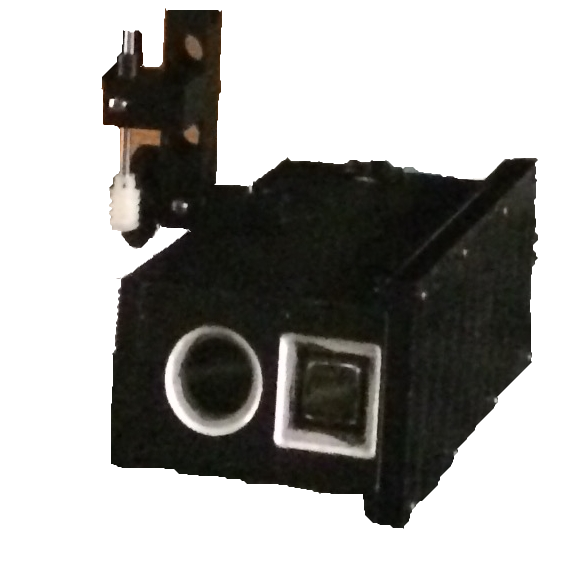
\includegraphics[scale=0.2]{OpticalBox.png}
%	\caption{Optical Box Sample}
%	
%\end{figure}

\subsection{Electronics and Primary PMT} 

*Refer to Appendix III for detailed electronics information

\subsection{Environment Management} 
In order to reduce variation between measurements and replicate the experimental conditions at Super-K and other neutrino detectors, the environmental variables, primarily temperature, ambient magnetic field, ambient light intensity and light transmission medium (water) must be controlled. 

\FloatBarrier

\begin{figure}[!htpb]
	\centering	
	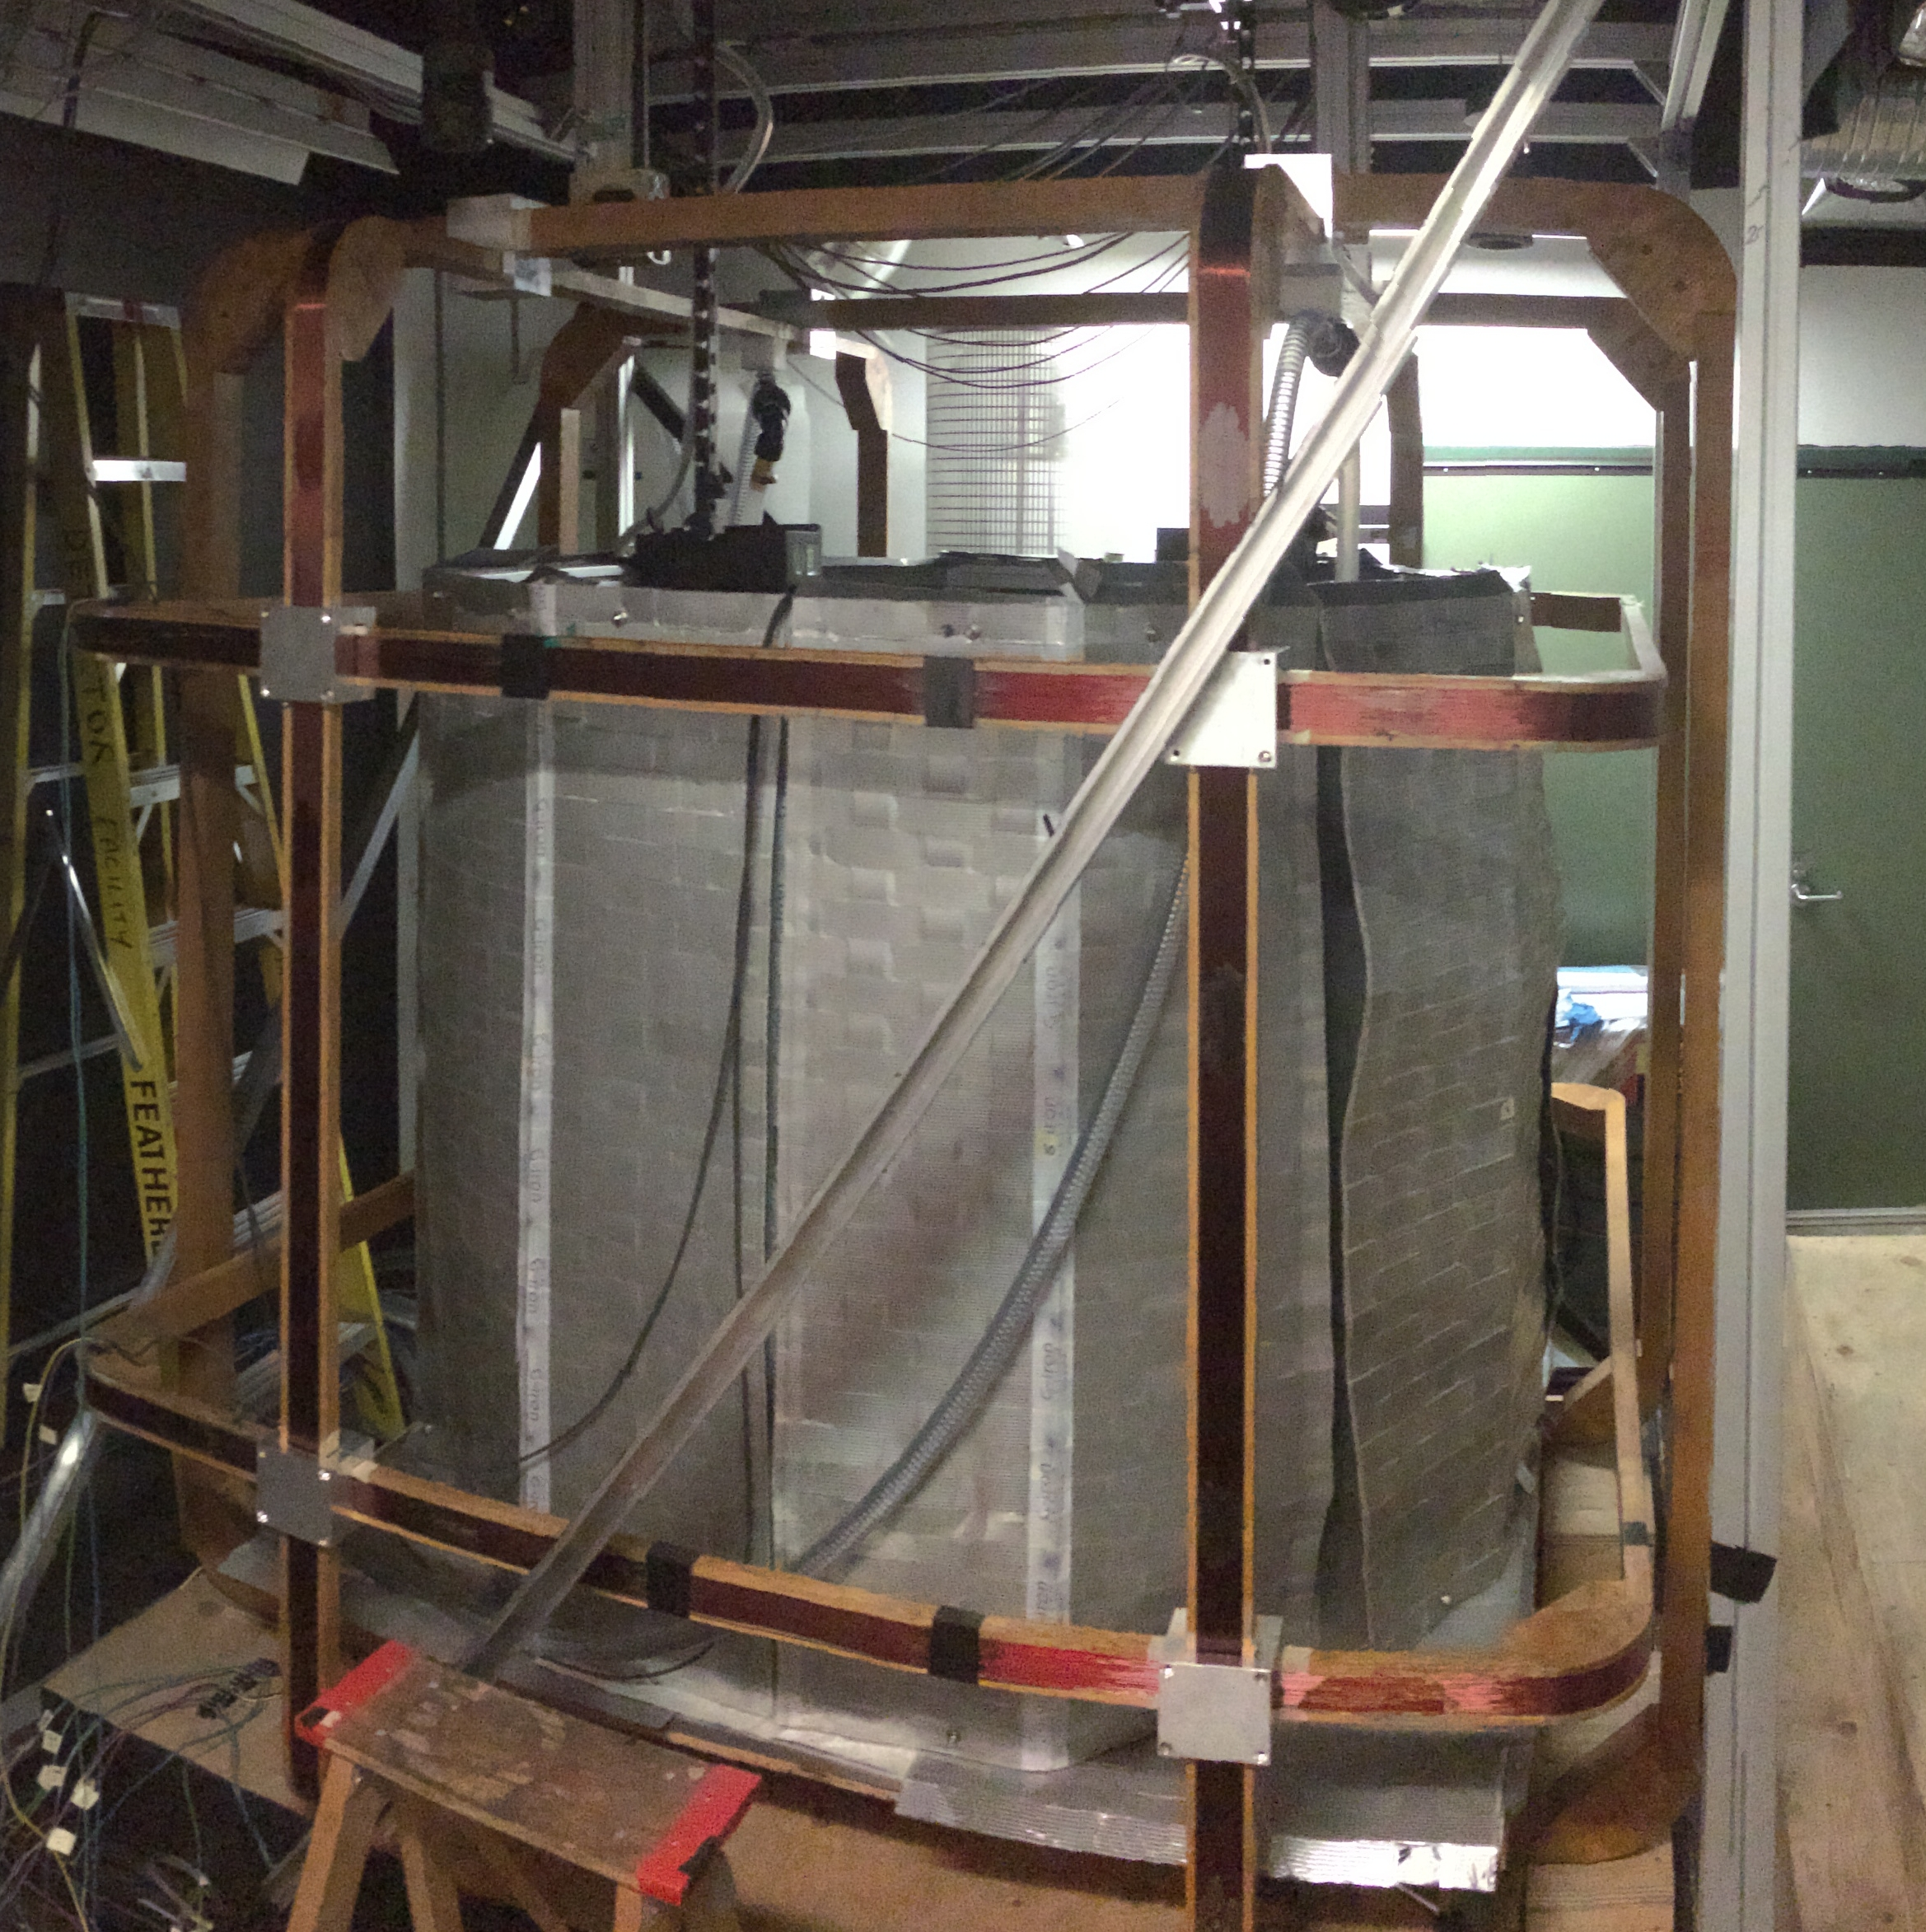
\includegraphics[scale=0.09]{PTF_w_a}
	\caption{Helmholtz Coil and Magnetic Shielding surrounding PMT in Tank}
\end{figure}

\FloatBarrier

\vskip 0.05in
\begin{description}
\item [Temperature Control]
Control of the temperature within the PTF is accomplished using a thermostat for the room attached to the central HVAC system.  The system is set to hold the temperature at $20\degree C$ with a cyclical variation observed of \texttildelow $1 \degree C$ (See appendix A).
\vskip 0.05in
\item [Magnetic Field Control]
The location of the PTF close to the cyclotron at TRIUMF necessitates control of the magnetic field using 3 pairs of Helmholtz coils surrounding the primary PMT.  The current in the coils is controlled by regulating the voltage applied.  Ideally, the coils reduce the magnetic field to $<100$ mG in all directions, however in practice this is difficult to achieve.  In addition to the coil compensation, there is a layer of G-Iron magnetic shielding around the primary PMT and underneath the water tank that houses the primary PMT. Current consideration is ongoing as to the benefit of the magnetic shielding (See Appendix A).
\vskip 0.05in
\item [Ambient Light Levels]
As the PMT is sensitive to single photons, it is important that the PMT be situated in a complete darkroom environment.  This is achieved with a combination of best practices and physical barriers.  The physical barrier to ambient light entering the PMT consists of a set of doubled curtains that enclose the entirety of the apparatus (i.e the Helmholtz coils, the water tank, and the primary PMT).  This barrier is sufficient to shield the apparatus on its own, however standard practice is to also turn off any ambient light sources. 
\vskip 0.05in
\item [Water System]
The production of Cherenkov light from neutrino interaction necessitates the use of very pure water as the optical medium in large scale water Cherenkov detectors such as Super-K and Hyper-K.  In order to accurately characterize the behaviour of the PMT in the PTF, all measurements must be taken in ultra-pure water.  The water is filtered through an active and passive filtration system for particulate and organic matter, such that it is to a good approximation the purity of the water used in Super-K and Hyper-K. The precise details of the system as well as a graphical representation of the flow can be found in Appendix $\alpha$ 
\end{description}

\subsection{Control Interface} 
The primary means of control of the apparatus is via a terminal, which can be remotely accessed from machines outside of the PTF. The machine hosts a status page from which a number of front-end programs are accessible.  These include programs to control the motion of the optical boxes and the high voltage power supply for the Helmholtz coils/PMTs, and various logging programs for tracking environmental and measurement data. A complete description of each of the programs as well as general instructions for their operation is included in Appendix C.
     
\section{Operation}

*See Appendix III for Standard Operating Procedures

\section{Analysis and Measurements}\label{sec:general_analysis}

\subsection{ADC Spectrum Analysis}\label{sec:adc-spectrum-analysis}
Upon incidence of a photon to the surface of the PMT, an electron is emitted into the PMT vacuum tube by the photoelectric effect and focused towards a series of dynodes which use the process of secondary emission to massively increase the number of electrons produced.  This increase is detected as an analog waveform, then integrated over a finite time period and converted to a digital signal using an Analog to Digital Converter (ADC), which can then write data to a file to be analyzed using a computer.  

The data written to file is in the form of a non-calibrated integer value that is linearly proportional to the total charge produced by the PMT. The constant of proportionality that defines this relationship must still be calculated. 

If many single photons are sent in sequence to the PMT over a finite time period, a distribution of ADC output is generated and binned into a histogram known as an ADC Spectrum. Characteristic of an ADC Spectrum is a narrow, sharp peak (ADC Pedestal) which corresponds to the integration of a waveform that does not contain an event, and a second, more broad distribition (PE Peak) which is composed of the ADC output from the integration of waveforms produced by a photon incident on the PMT surface. 
\FloatBarrier

\begin{figure}[!htpb]
	\centering	
	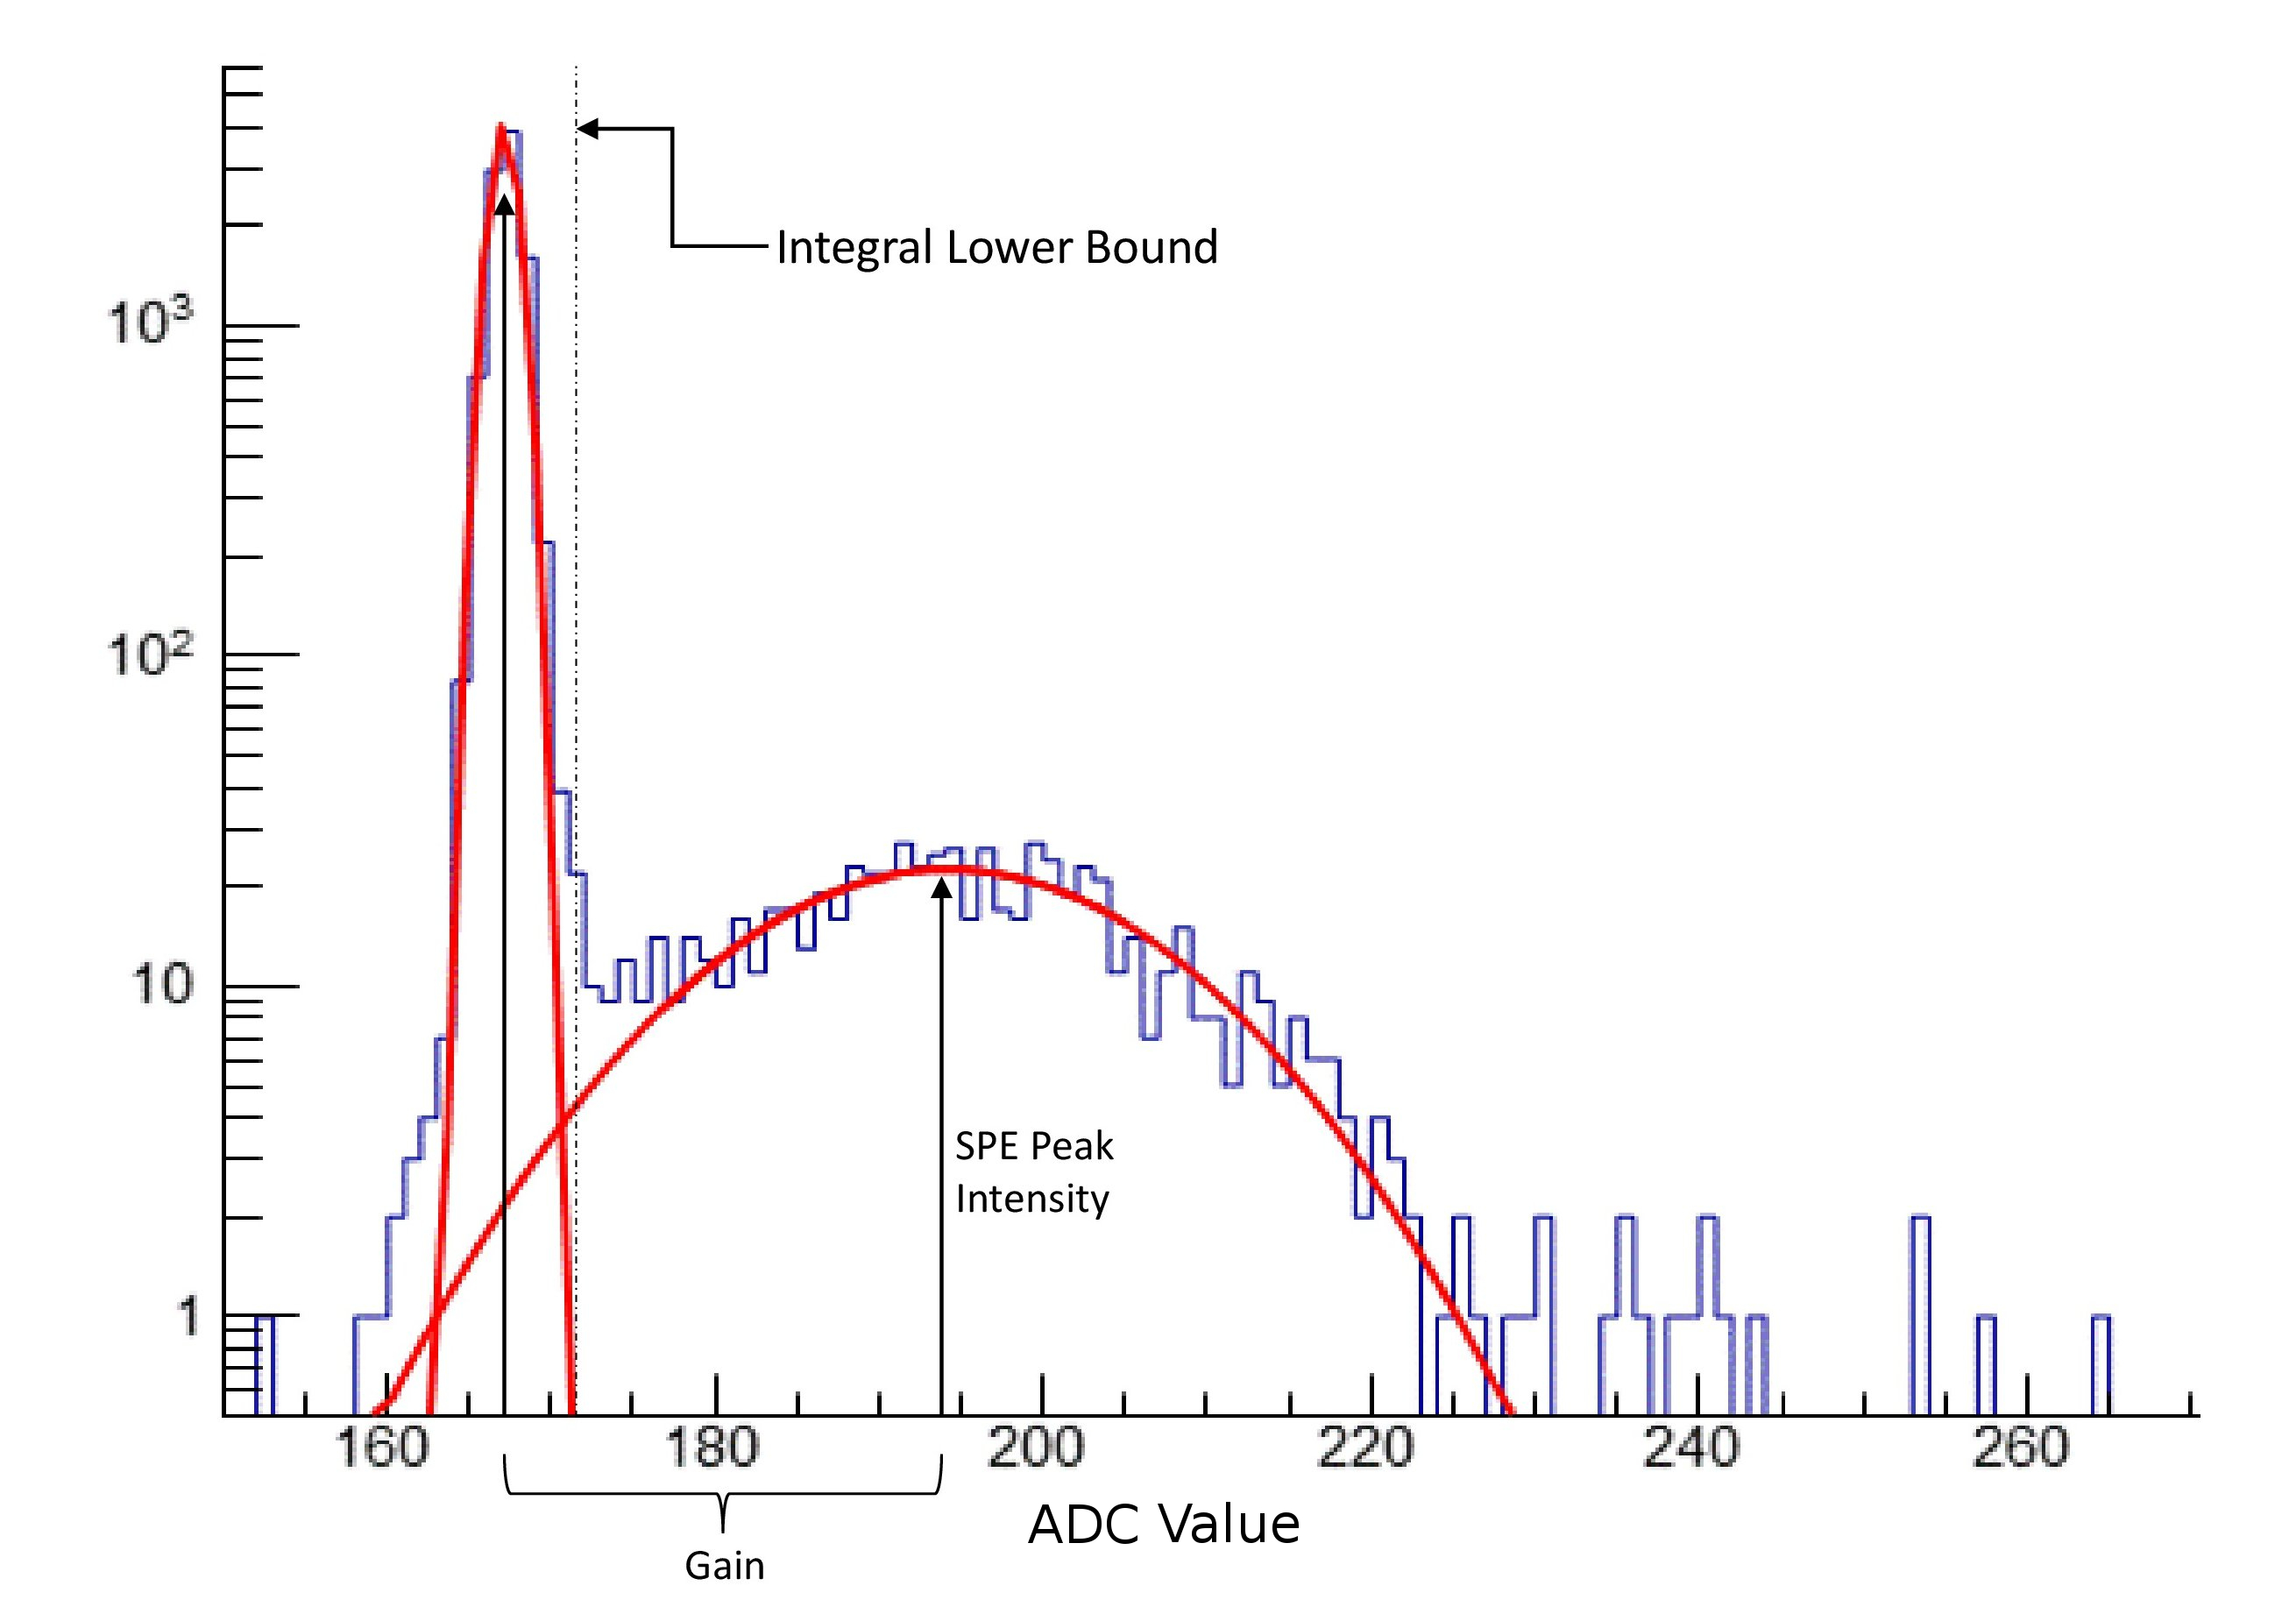
\includegraphics[scale=0.09]{exampleSpectrum.jpg}
	\caption{Sample ADC Spectrum with Labels}
	
\end{figure}

\FloatBarrier

Extraction of PMT response characteristics from an ADC Spectrum is accomplished through fitting of both the ADC Pedestal and PE Peak distributions with Gaussian functions and manipulating the direct fit result data, such as Peak Intensity, Spread (Sigma), and mean value.  Additional characteristics can be obtained by utilising secondary fit data, including the integral of each distribution, the difference function between the two gaussians, etc.

\begin{description}

\item[Gain]
The gain of the PMT at a point on its surface is the amount of charge in ADC counts measured relative to the amount of charge measured for a no event signal.  To extract the gain from the ADC Spectrum, the mean of the fitted Pedestal gaussian is subtracted from the mean of the fitted PE Peak gaussian. Further discussion of results from gain studies conducted can be found in Section $\chi$
\vskip 0.05in
\item[Peak Intensity]
The Peak Intensity refers to the height of the fitted PE Peak Gaussian.  This parameter can be directly extracted from fitting the gaussian.
\vskip 0.05in
\item[Detection Efficiency]
The overall detection efficiency of the PMT at a point is calculated by determining the intersection point of the Pedestal and PE Peak gaussian fits, and integrating over the ADC Spectrum with the exception of the data points which comprise the Pedestal.  This integral corresponds to the number of detected photoelectrons (assuming Single PE Peaks), and dividing by the total number of incident laser pulses (photons) yields a measure of the overall detection efficiency.
\vskip 0.05in

\item[Charge Resolution]
The charge resolution of the PMT at a point is calculated as the quotient of Peak Intensity and spread of the fitted Gaussian (Sigma).
\vskip 0.05in

\item[Peak To Valley Ratio]
The peak to valley ratio is defined as the ratio between the height of the PE Peak (Intensity), and the height of the local minimum between the Pedestal and the PE Peak.  In terms of extracted parameters, the Peak to Valley ratio can be calculated as the intensity of the PE Peak divided by the height of either fitted gaussian function at the local minimum of the difference between the PE Peak gaussian and the Pedestal gaussian.

\end{description}
\vskip 0.05in

Analysis of the ADC Spectrum from a range of points and incidence angles on the PMT surface is the primary means of characterizing the response of the PMT, and as such the development of tools to rapidly and automatically analyze ADC Spectra across the entire PMT surface is crucial. The analysis tools for the PTF are written primarily in C using the ROOT library as the framework for data analysis and plotting.  ROOT is an open source, fully featured software library for use with C and C++ developed at CERN, and provides a suite of powerful tools for research and High Energy Physics applications. 

Data collected with the ADC for a given laser pulse is stored in a MIDAS file with a variety of parameters that specify the position of the gantry during the measurement, the number of pulses that compose the measurement, the magnetic field magnitude during the measurement and the magnetic field compensation coil settings.  For a run that is comprised of measurements at various gantry positions, the system also assigns an index to each position and the corresponding number of measurements made at each position.  The MIDAS file is compiled into a ROOT file (hierarchical in structure) and the file is iterated over with a ROOT script to generate an ADC spectrum for each gantry position. 
*Refer to Appendix III for complete ADC Spectrum analysis algorithm and sample code

The resulting ADC spectrum for each gantry position is fitted with gaussian functions over the range of the Pedestal and the PE Peak, and a single parameter is extracted and binned into a 3d histogram, the bins of which correspond to a position on the X-Y plane of the PMT.  A range of positional resolutions can be used, the smallest being $2mm$. Once the complete ROOT file is iterated over, a plot of the extracted parameter is contained in the 3d histogram and can be displayed.  

\FloatBarrier

\begin{figure}[ht]
	\centering	
	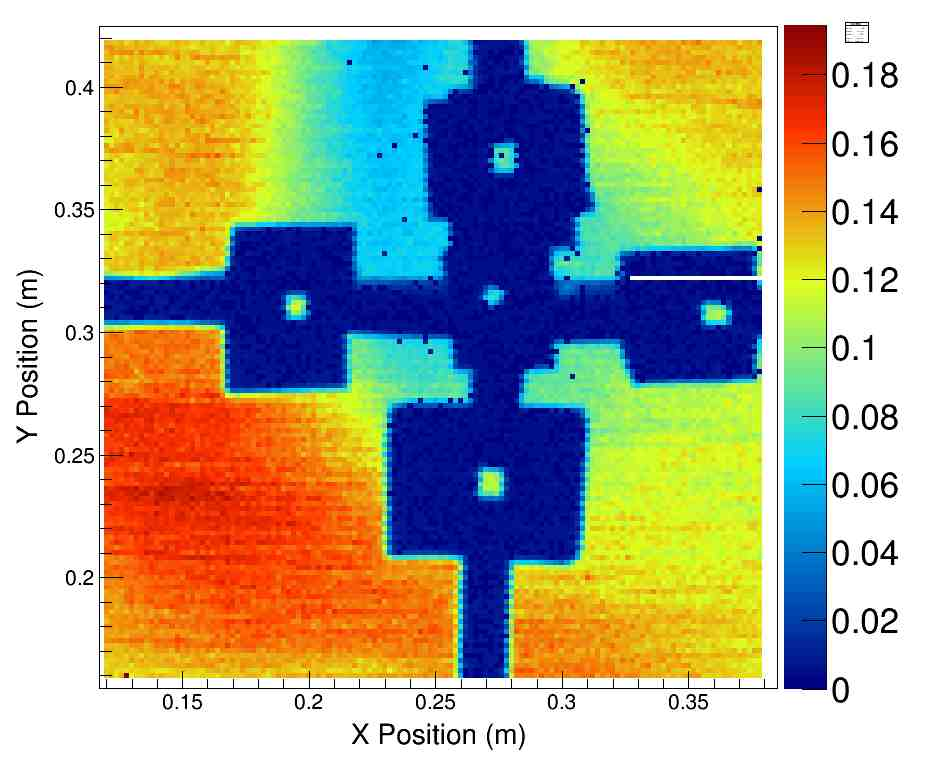
\includegraphics[scale=0.19]{relative_detection_efficienty.jpg}
	\caption{Relative Detection Efficiency Scan: 2mm Resolution with Gantry 0}
\end{figure}

\FloatBarrier

Additional histograms are also constructed providing 2D distributions of parameters such as gain, intensity and peak to valley ratio for all measurements. As well, for each fitted gaussian, a $\chi^2$ goodness of fit metric is calculated and the quotient of $\chi^2$ and the number of degrees of freedom required for the fit is plotted in a histogram.  These additional plots are compiled into a figure and displayed alongside the 3D histogram generated from the ADC Spectrum analysis.      
\vskip 0.05in

\FloatBarrier

\begin{figure}[!htpb]
	\centering	
	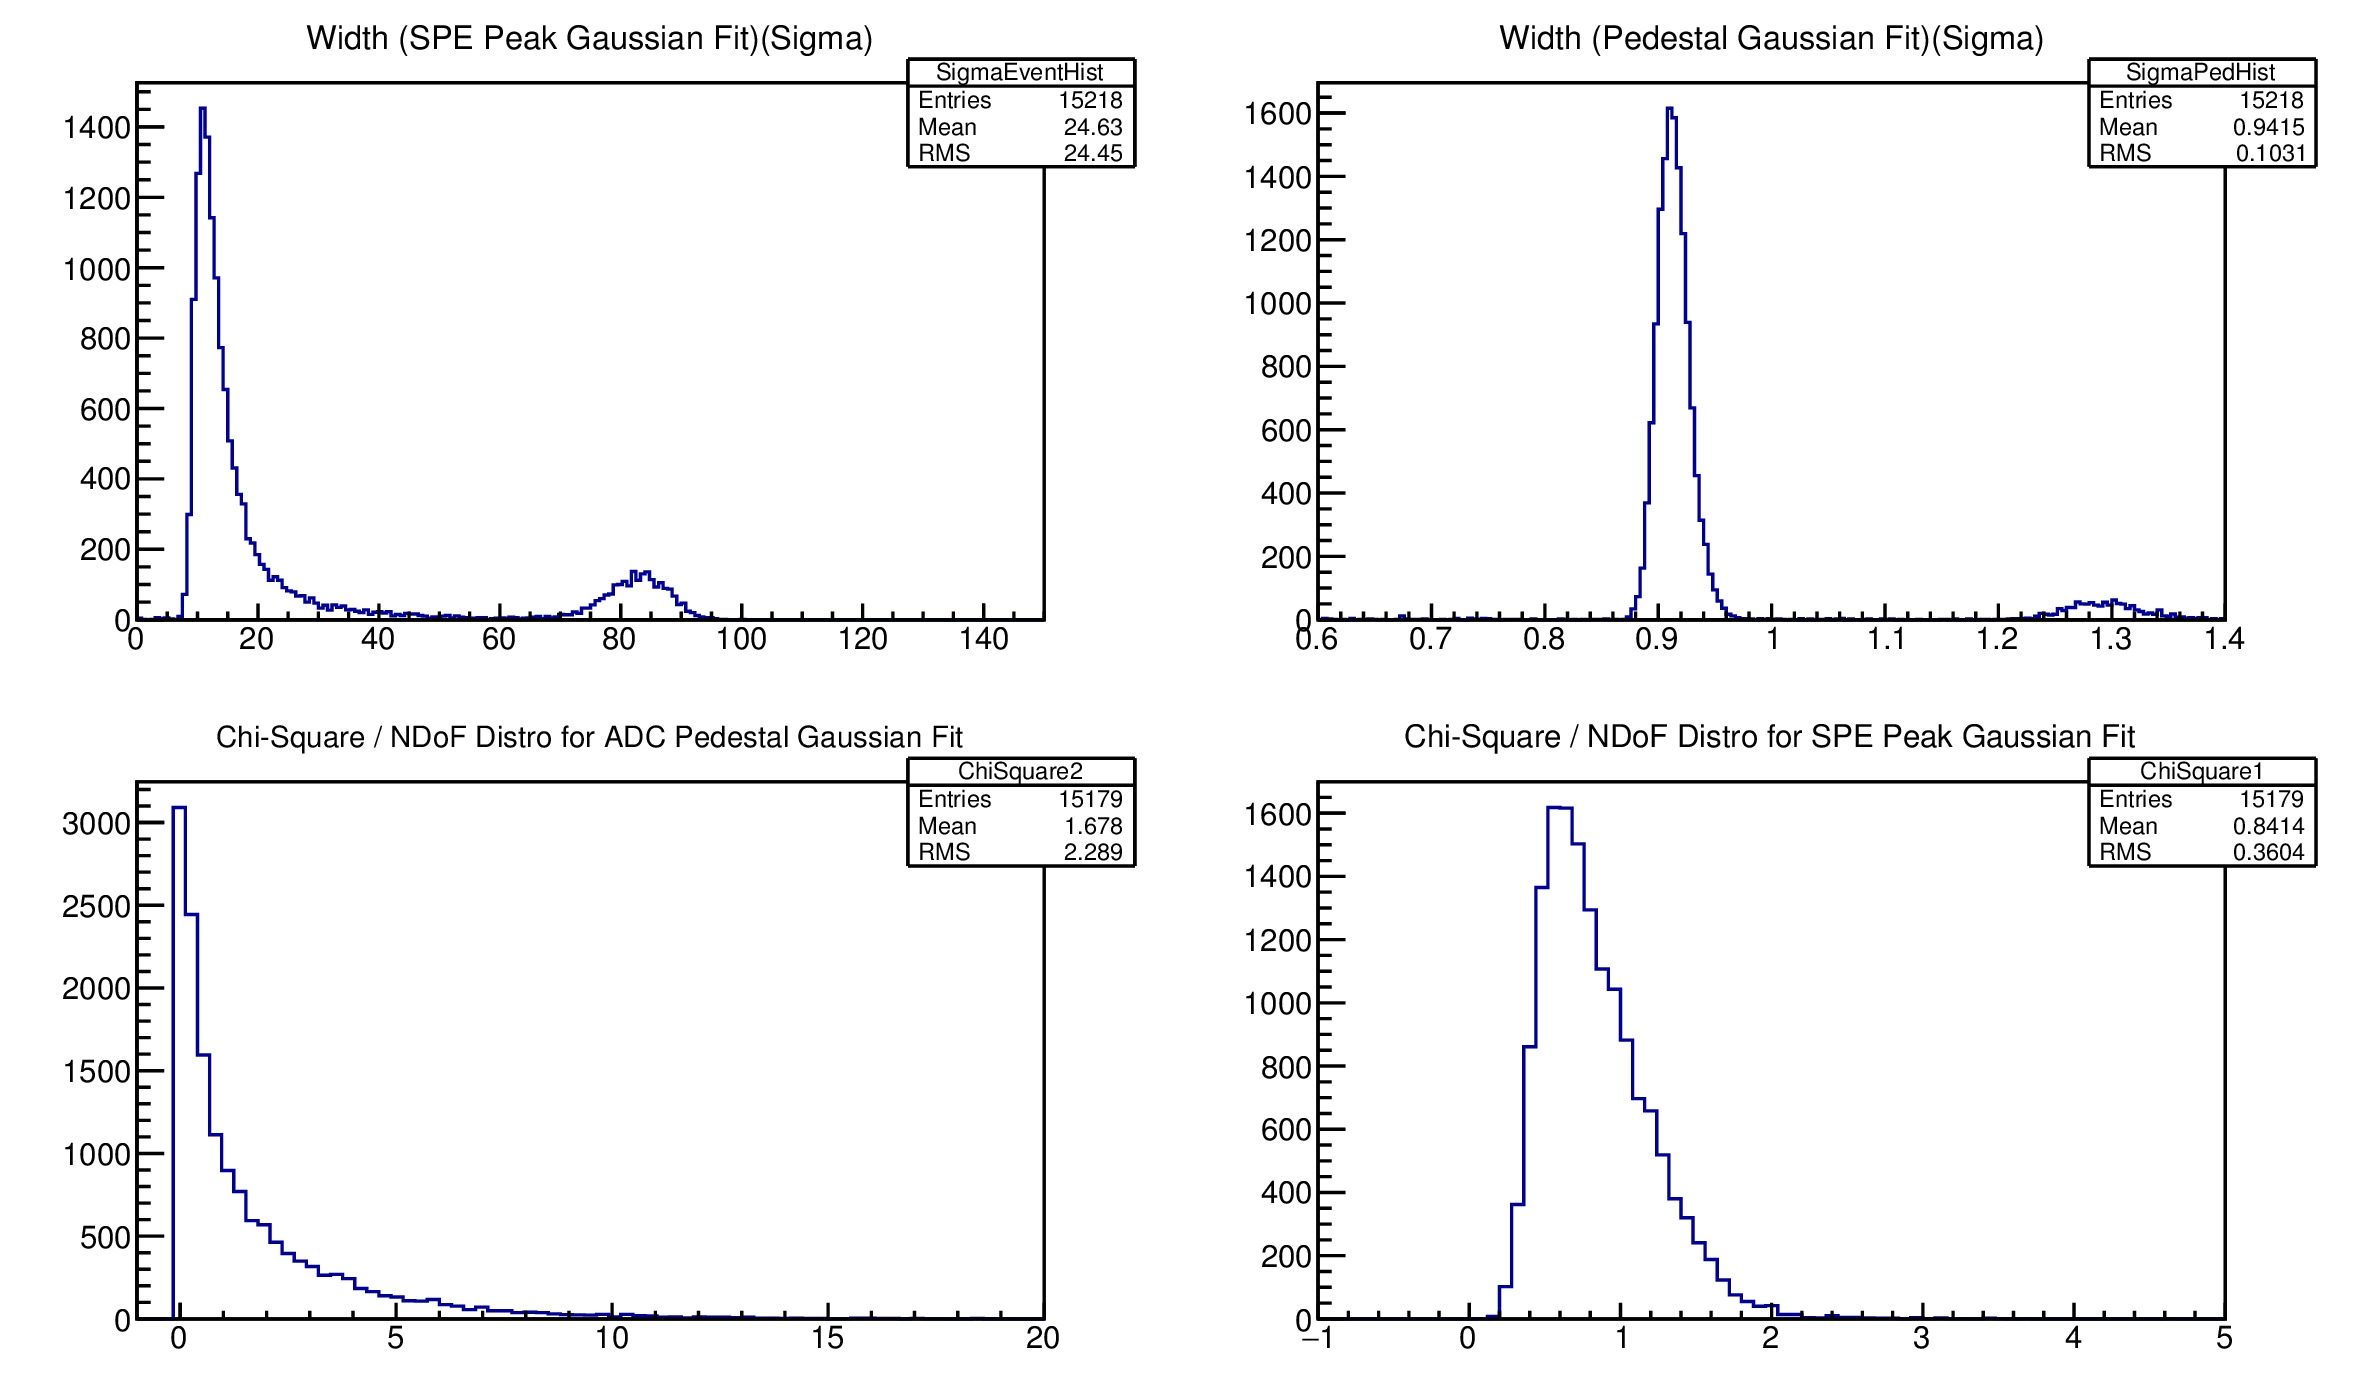
\includegraphics[scale=0.4]{exampleStats.jpg}
	\caption{Extracted Fit Parameters and Goodness of Fit Metrics (5mm Scan)}
	
\end{figure}

\FloatBarrier

\subsection{Environmental Data Collection}

Inside of each optical box, there is a small chip (Phidget) capable of measuring the magnetic field, acceleration and tilt of each optical box.  Data from these phidgets is collected during gantry motion and the data can be extracted and plotted in a 3D histogram in the same way as any of the other extracted parameters (gain, intensity etc.). This enables quantitative measurement of the effect of magnetic field on the response of the PMT. 

\FloatBarrier

\subsection{Incidence Angle Control} \label{sec:incAngle}



The 5-axis gantry system enables control of incident photons to a specific point on the PMT surface at a range of incidence and azimuth angles (refer to figure with incidence and azimuth explanation). Accurate positioning of the laser beam on the surface is obtained through a careful calibration of the gantry system and precise measurement of the location of the PMT within the gantry coordinate frame. 

Due to the 5 degrees of freedom of the gantry system, calculation of the position of the optical box which yields a beam of photons incident to a desired position on the PMT at a desired incidence and azimuth angle is non-trivial. The script which handles the calculation is written in Python and performs the calculation according to the algorithm detailed in \ref{incidence}. Sample code implementing the algorithm is contained in the Appendix.

\begin{algorithm}[!htpb]
\caption{Gantry Position Incidence Algorithm}\label{incidence}

\KwIn{x,y position of PMT center, x,y offset of point from PMT center, laser beam length, incidence angle, azimuth angle, radius of PMT spherical cap}
%Input of initial values

\KwOut{Final x, y, z position, tilt angle, rotation angle with suggested gantry}

Calculate corresponding z position for point at x,y on PMT surface assuming spherical cap
%Creation of angles describing rotation in PMT Frame

Define normal direction in spherical angles to surface of PMT at x,y

Convert x,y to Gantry coordinate frame by superposition of x,y of PMT center and x,y offsets
%Spherical to Cartesian

Convert spherical coordinates defined by laser beam length, incidence angle and azimuth angle to cartesian coordinates.

%Rotation about y axis of PMT

Rotate cartesian coordinates from $\bm{4}$ so the z-axis is co-linear with the direction defined in $\bm{2}$ and the x-axis is normal to the 2-D projection of the PMT surface in x,y

%Superposition of Coordinates

Add rotated cartesian coordinates to x,y position calculated in $\bm{3}$ to obtain ideal point source coordinates

Calculate final rotation and tilt angles in gantry frame from vector between ideal point source coordinates in $\bm{6}$ and surface point coordinates in $\bm{3}$

Obtain the perpendicular offsets to the laser beam from the gantry tilt and rotation axes for each gantry

\eIf{$\lvert Gantry\ Rotation\ Angle\rvert < 2\pi/3$}{
	Decide to use gantry 0 as active gantry
	
	From final rotation and tilt angles in $\bm{7}$, calculate actual offsets in x, y, and z from rotation and tilt of gantry 0
	
	Calculate final gantry position from superposition of coordinates in $\bm{6}$ and gantry 0 offsets
	
	Add $\pi$ to the rotation of gantry 0
}{
	Decide to use gantry 1 as active gantry
	
	From final rotation and tilt angles in $\bm{7}$, calculate actual offsets in x, y, and z from rotation and tilt of gantry 1
	
	Calculate final gantry position from superposition of coordinates in $\bm{6}$ and gantry 1 offsets
}

\KwResult{Final x, y, z, rotation, tilt and suggested gantry}

\end{algorithm}
\FloatBarrier
\subsection{Location of PMT}

Location of the PMT in X and Y coordinates of the gantry system is achieved by placing a set of at least two temporary, simple markers on the surface of the PMT or on any material covering its surface.  One of these markers must be located at the center of the PMT, with another positioned at another point approximately $8cm-10cm$ away and ideally located such that the line between that point and the center point is parallel to either the X or Y axis of the gantry system. After placement of the markers, a scan of the PMT area is conducted at 2mm resolution wth the optical box oriented such that the laser beam is aligned with the gantry Z-axis (in layman's terms, pointed straight down).

Data from the scan is analyzed as per section \ref{sec:adc-spectrum-analysis}, and a plot of overall detection efficiency is generated. If the data collection and analysis system work correctly, the overall detection efficiency plot should clearly show the two markers on the surface of the PMT.  From the detection efficiency plot, the position of the central marker in the gantry coordinate frame is obtained, as well as the orientation of the PMT and the offset in position from the center of the second marked point. The uncertainty in these positions is $\pm1mm$.  

Location of the PMT in the Z-axis occurs in two steps:

\begin{enumerate}
	\item Rough location of the PMT in Z.  The z position of the top of the PMT is estimated in the gantry coordinate system to within 5cm and recorded as an initial calibration point.
	\item Scan sequence to accurately position the PMT in Z.  Using a spherical cap model of the surface of the PMT and the offset between the two markers placed on the PMT, calibration of the Z position of the PMT can be achieved. Using the roughly estimated Z position as an input, the required gantry position to achieve photons incident at the non-central marked point is calculated for a range of incidence angles ($-20\degree, -10\degree, 0\degree, 10\degree, 20\degree$). 
	
	A $4cm\times4cm$ area scan at $2mm$ resolution as detailed in \ref{sec:adc-spectrum-analysis} is conducted for each of these gantry positions with the calculated X and Y position used as the center of the scan and the rotation, tilt and Z positions of the gantry kept constant. Each scan is analyzed for overall detection efficiency and the position of the second taped marker is recorded (additional unique markers may be required for positional determination if the second taped marker does not appear at some incidence angles).
	
	Using the coordinates of the second taped marker in each scan and the offset from the actual location of the second marker, the offset in Z position from the surface point on the PMT to the focal point of the laser can be calculated.  Correcting for the offset such that the focal point of the laser is located on the surface of the PMT at the second taped point is sufficient to calibrate the system to an accuracy of ... 
	\Todo{Add uncertainty from tilt and xyz positioning}  
	
\end{enumerate}
The process of locating the PMT must be completed separately for each optical box, as the two optical boxes do not share a common coordinate system.  Once the position of the PMT is known in each gantry frame, quantitative uncertainties in the position of the laser spot and incidence/azimuth angles are calculable for measurements taken with each optical box. 

\section{Observations}

Using the methods described in section \ref{sec:general_analysis} as a framework for data collection and analysis, a number of preliminary studies regarding a range of PMT characteristics were conducted.  These studies served as both a test of equipment and analysis methods, and provided a starting point for further investigations.

\subsection{PMT Response}

A number of full area scans were taken at 5mm and 1cm resolutions (as per section \ref{sec:general_analysis}) in the X-Y plane with each optical box, with motion constrained to the plane $z = 0.35m$.  The rotation and tilt of the optical boxes were both set at $-90\degree$ and kept constant throughout the scans.   
\FloatBarrier

\begin{figure}[!h]
	\centering	
	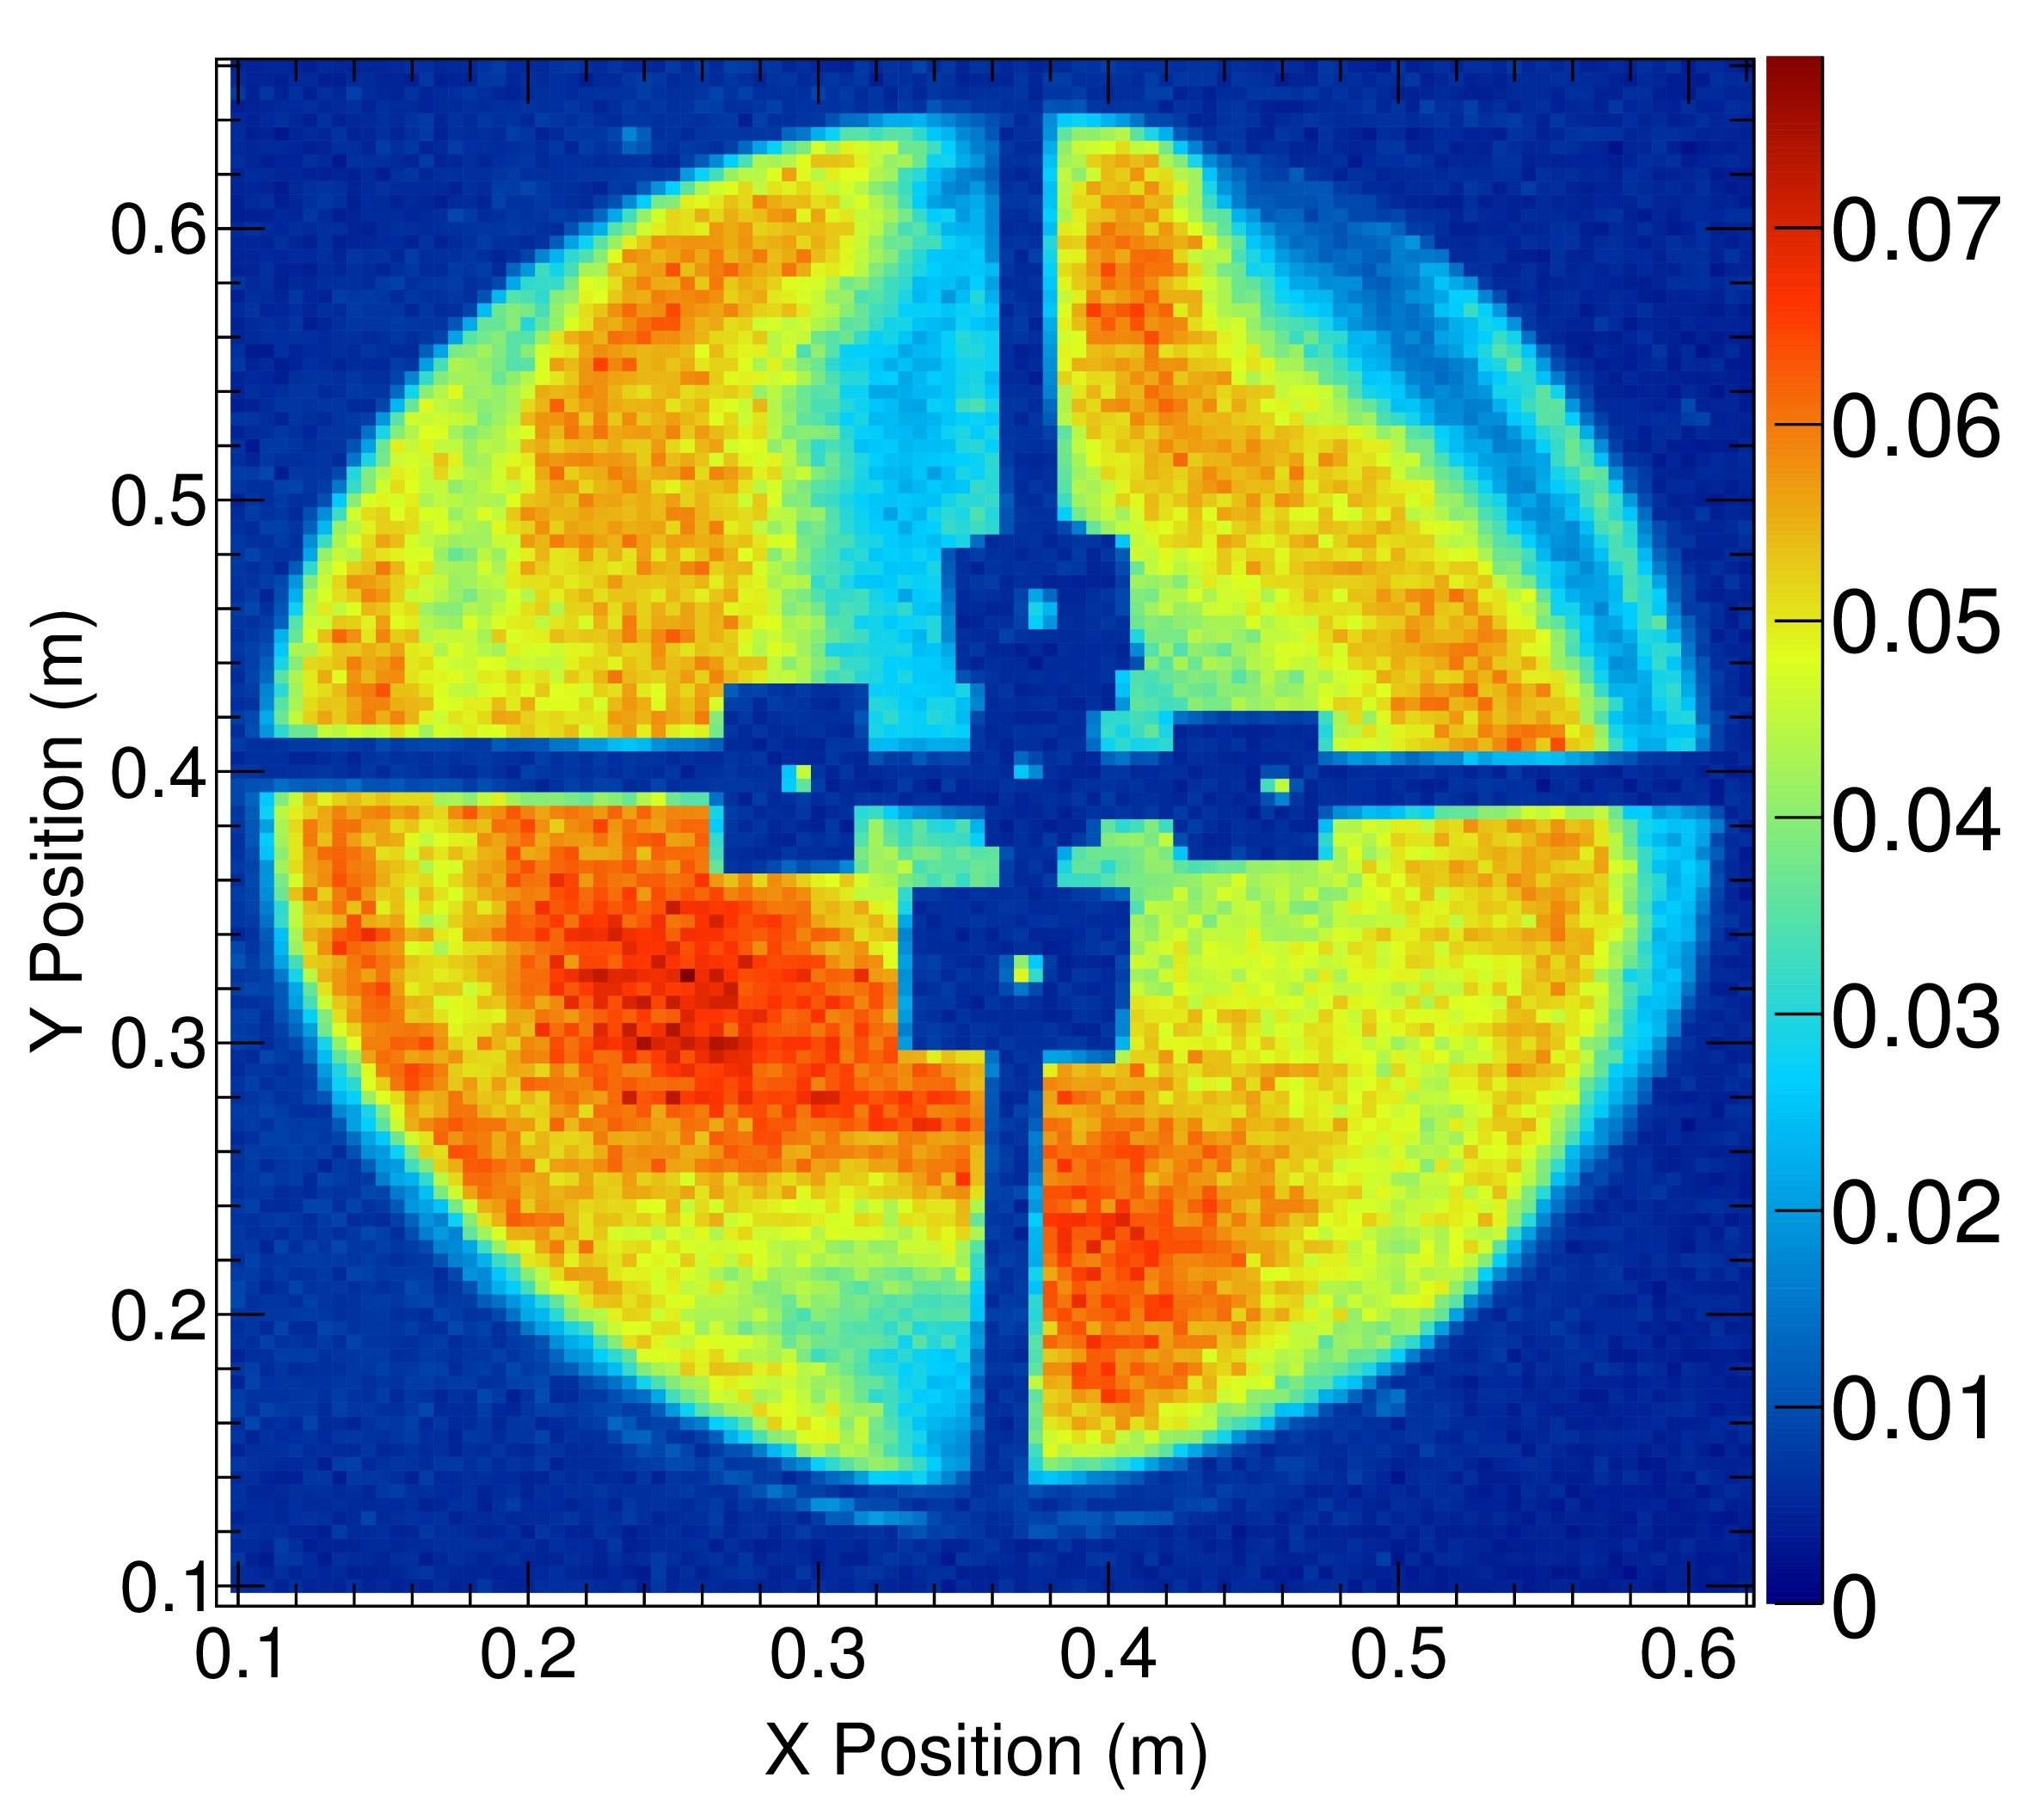
\includegraphics[scale=0.085]{relative_detection_efficiency5mmOld.jpg}
	\caption{Relative Detection Efficiency Scan (5mm Resolution)}
\end{figure}
\FloatBarrier
\begin{figure}[!htpb]
	\centering	
	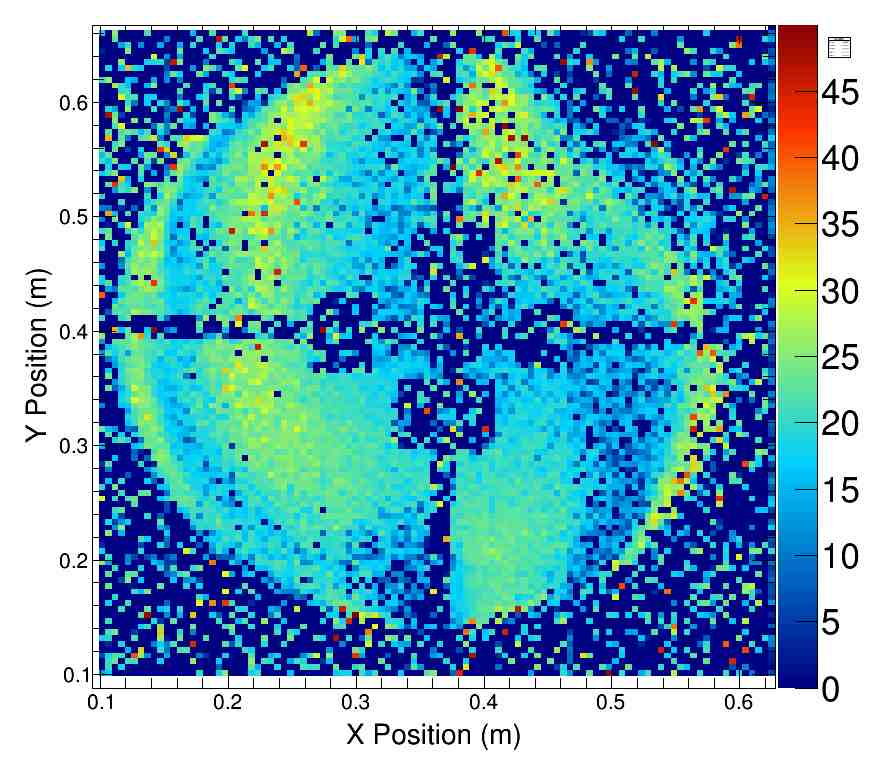
\includegraphics[scale=0.22]{5mm_gain.jpg}
	\caption{Gain Scan (ADC Count) at 5mm Resolution}
\end{figure} 
\FloatBarrier
\begin{figure}[!htpb]
	\centering	
	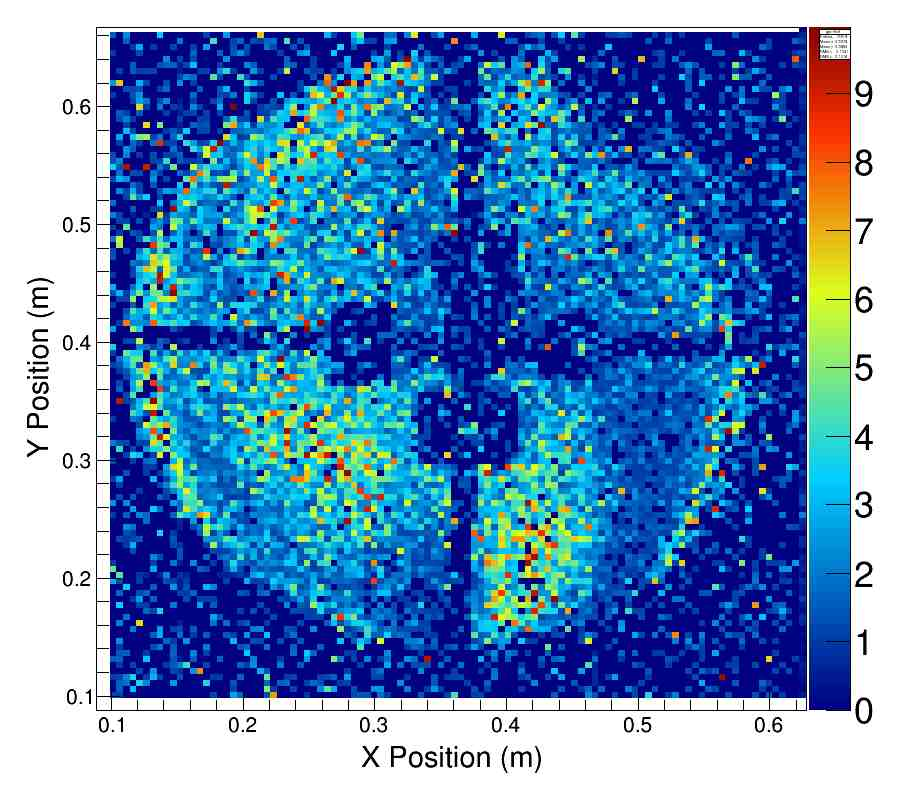
\includegraphics[scale=0.22]{5mm_pv.jpg}
	\caption{Peak to Valley Ratio at 5mm Resolution}
\end{figure}
\FloatBarrier
\begin{figure}[!htpb]
	\centering	
	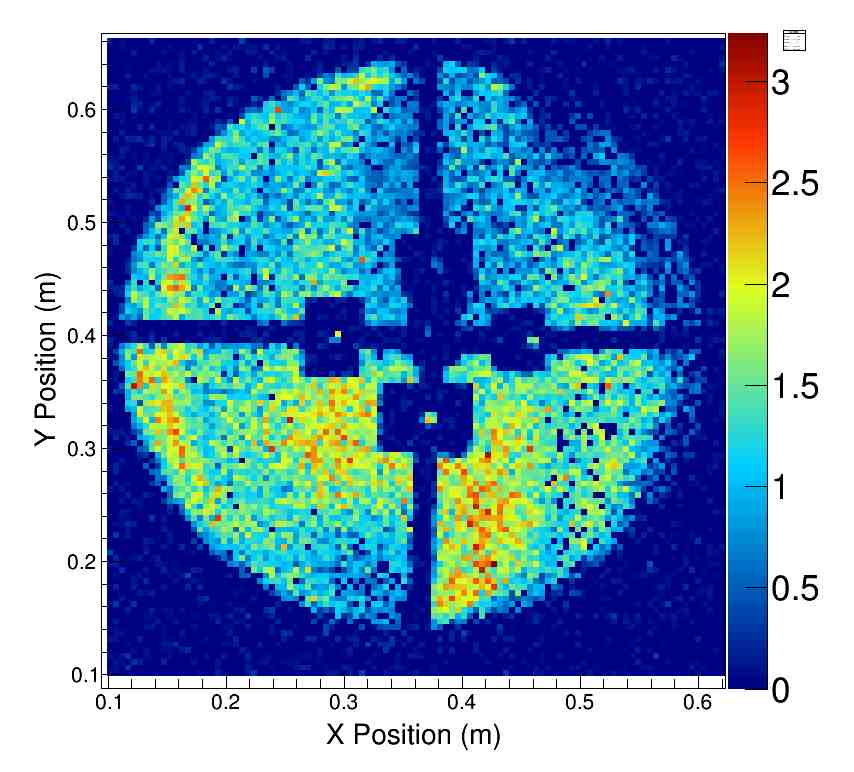
\includegraphics[scale=0.22]{5mm_cr.jpg}
	\caption{Charge Resolution at 5mm Resolution}
\end{figure}
\FloatBarrier

FIgures 5,6,7 and 8 show the results of these preliminary scans. 

Additionally, two scans at 1cm resolution were taken at opposite high ambient magnetic fields, with the field direction oriented along the Z-axis. Figures 9 and 10 show the results of these scans analyzed using methods described in \ref{sec:general_analysis}.

\FloatBarrier
\begin{figure}[!htpb]
	\centering	
	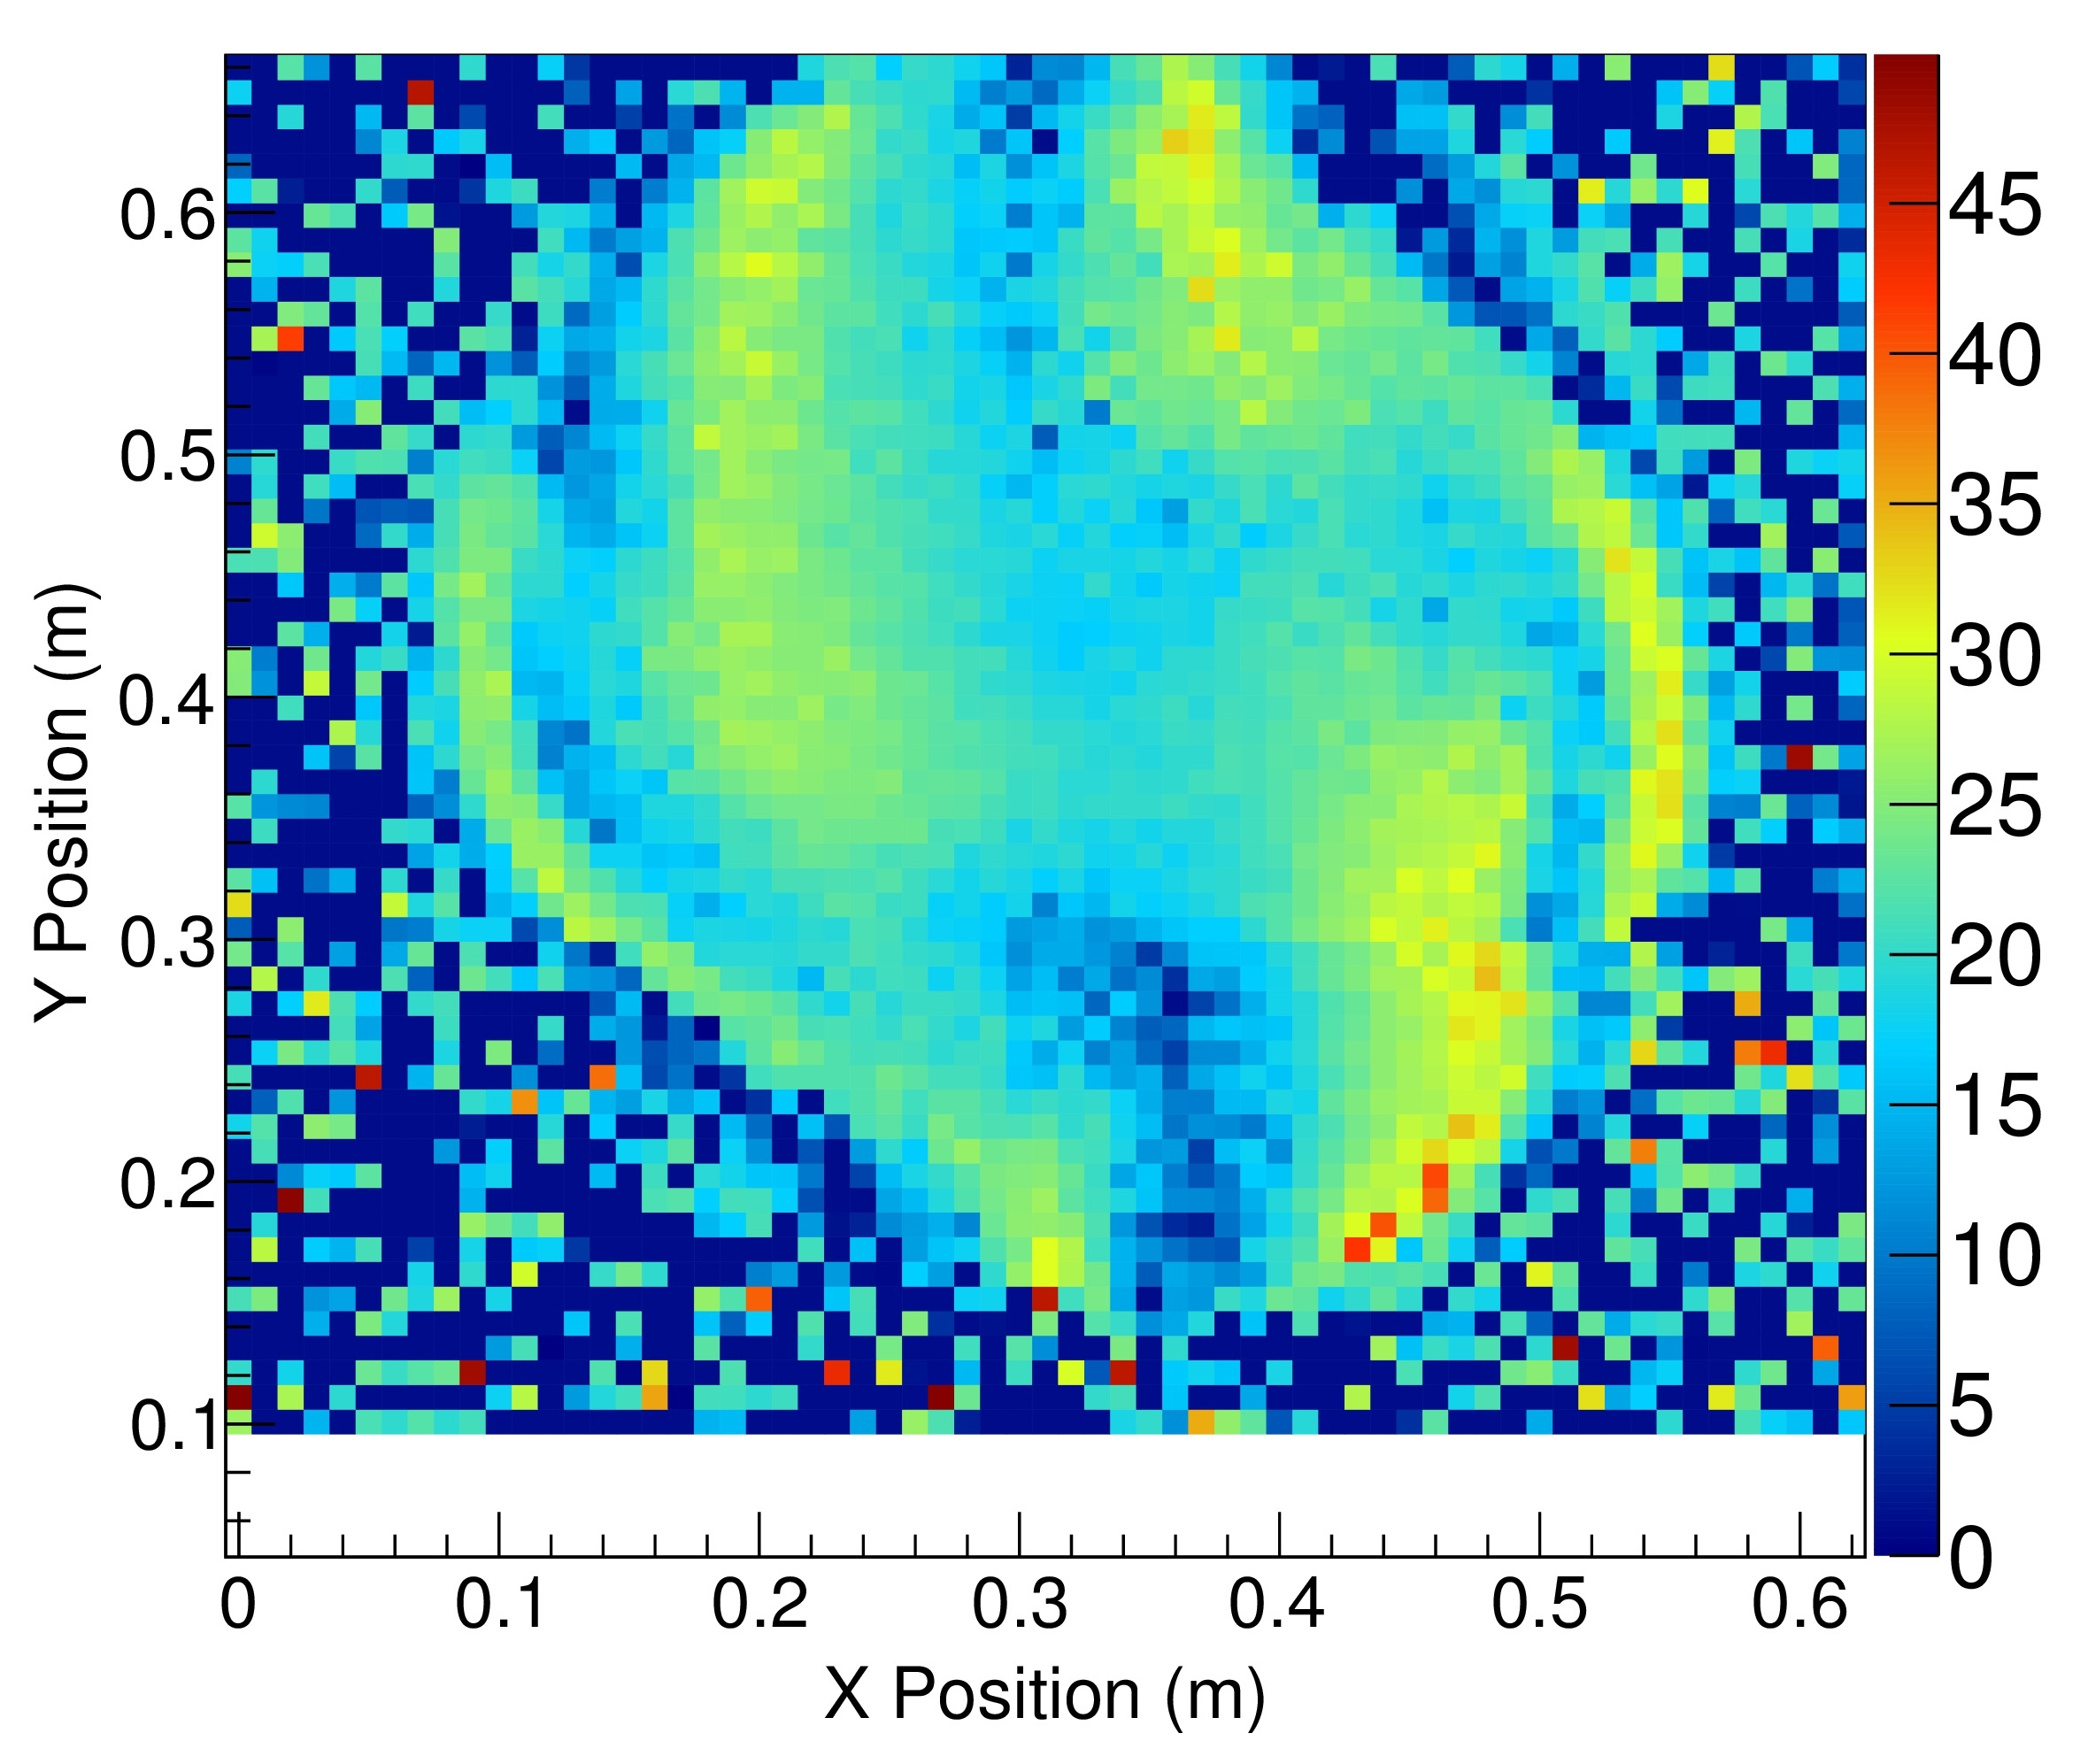
\includegraphics[scale=0.08]{gain_1456.jpg}
	\caption{Gain Scan at 1cm resolution with $+700mG$ field in Z-Direction}
\end{figure}
\FloatBarrier
\begin{figure}[!htpb]
	\centering	
	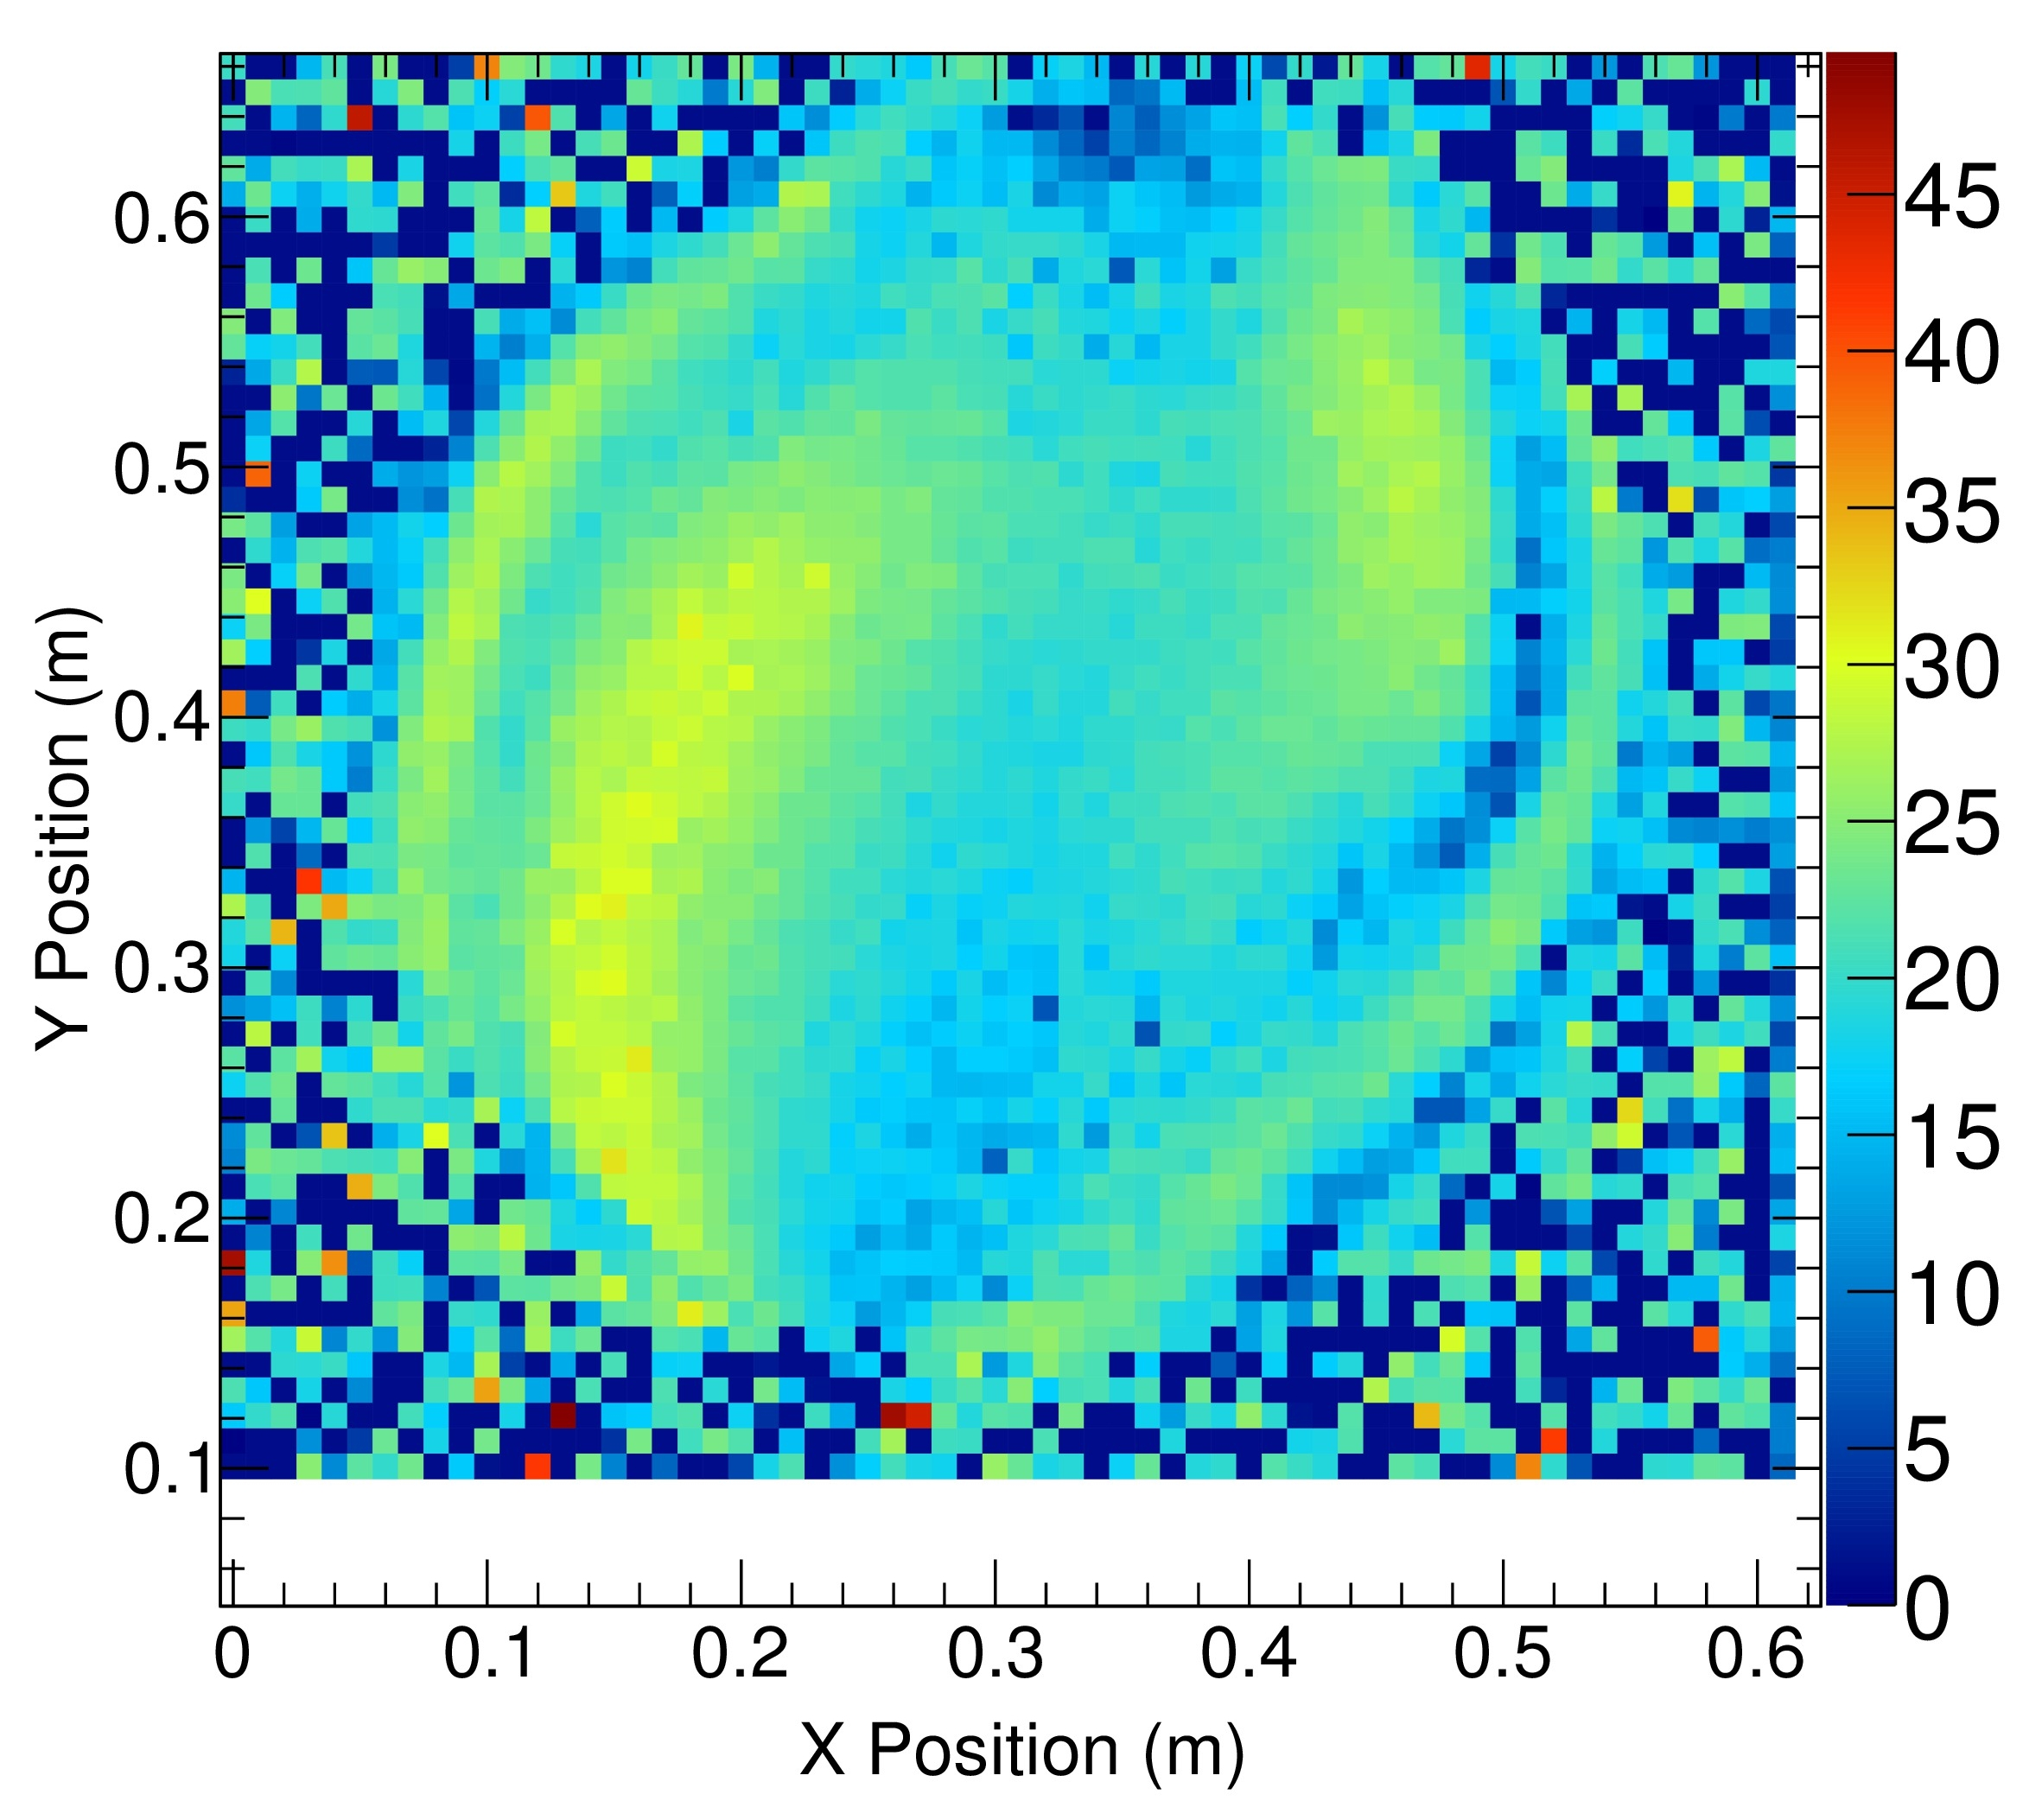
\includegraphics[scale=0.08]{gain_1466.jpg}
	\caption{Gain Scan at 1cm resolution with $-700mG$ field in Z-Direction}
\end{figure}
\FloatBarrier


\subsection{Incidence Angle Studies}

Preliminary investigation of the effect of incidence angle of the laser to the PMT was conducted manually while the incidence angle calculation script was being developed.  Data was collected for both gain and SPE Peak Intensity at a range of incidence angles at a single point. Figures 11,12 and 13 show the results of these measurements.

\FloatBarrier
\begin{figure}[!htpb]
	\centering	
	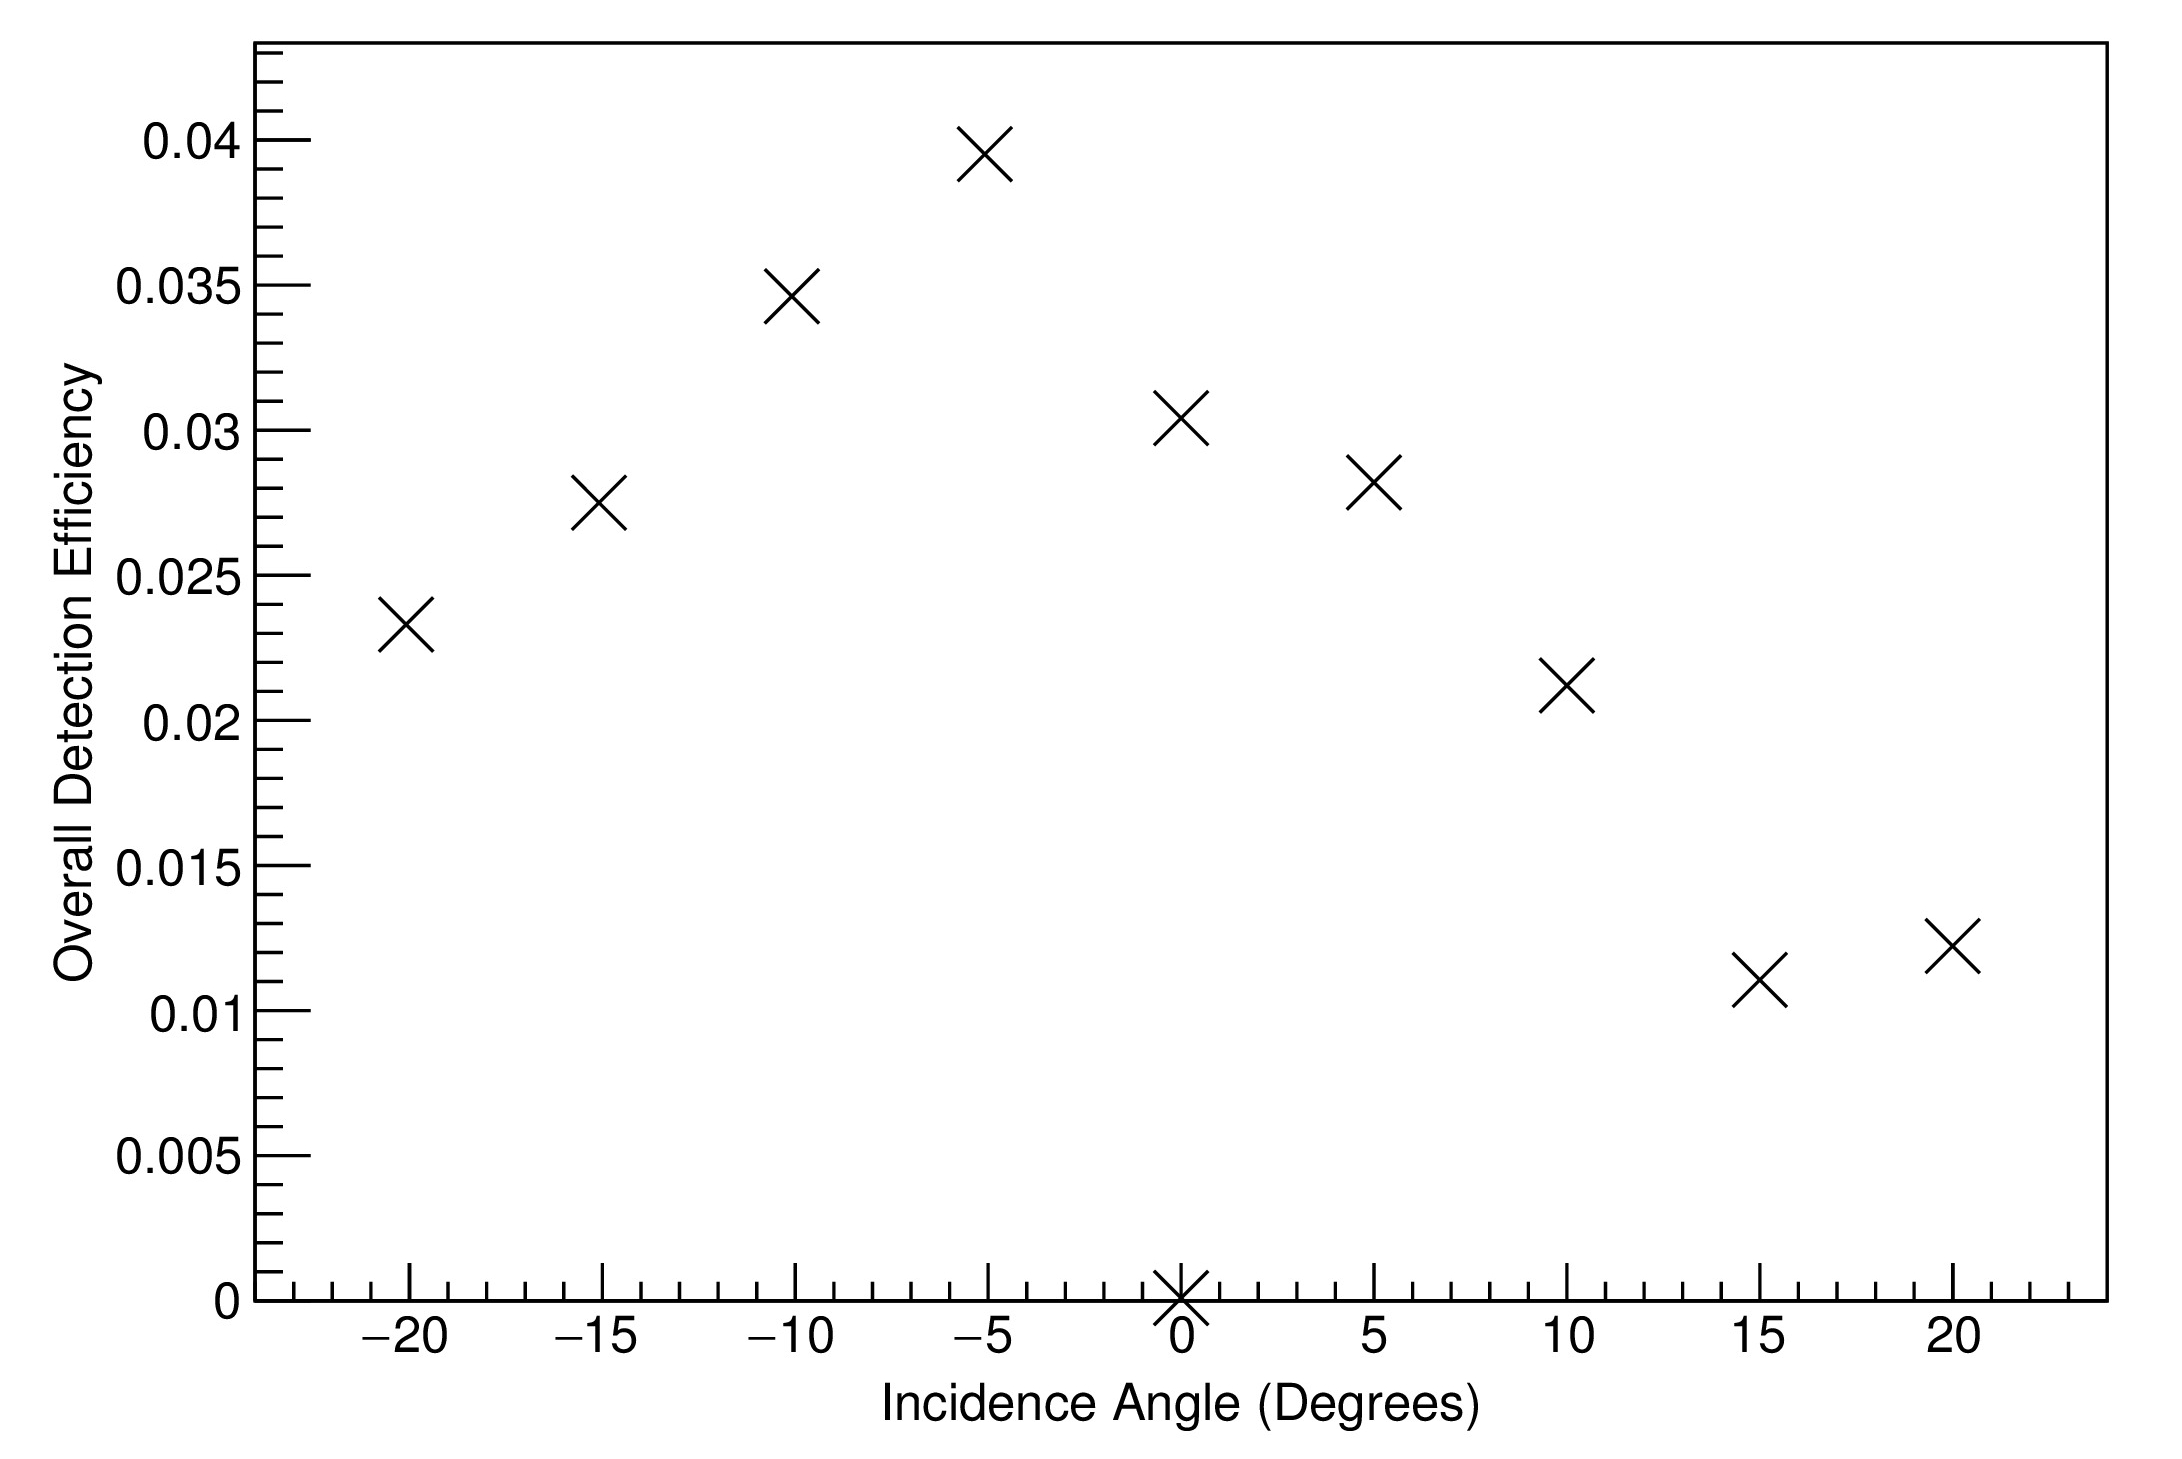
\includegraphics[scale=0.08]{detEffAngle.jpg}
	\caption{Detection Efficiency variation with Incidence Angle}
\end{figure}
\FloatBarrier
\begin{figure}[!htpb]
	\centering	
	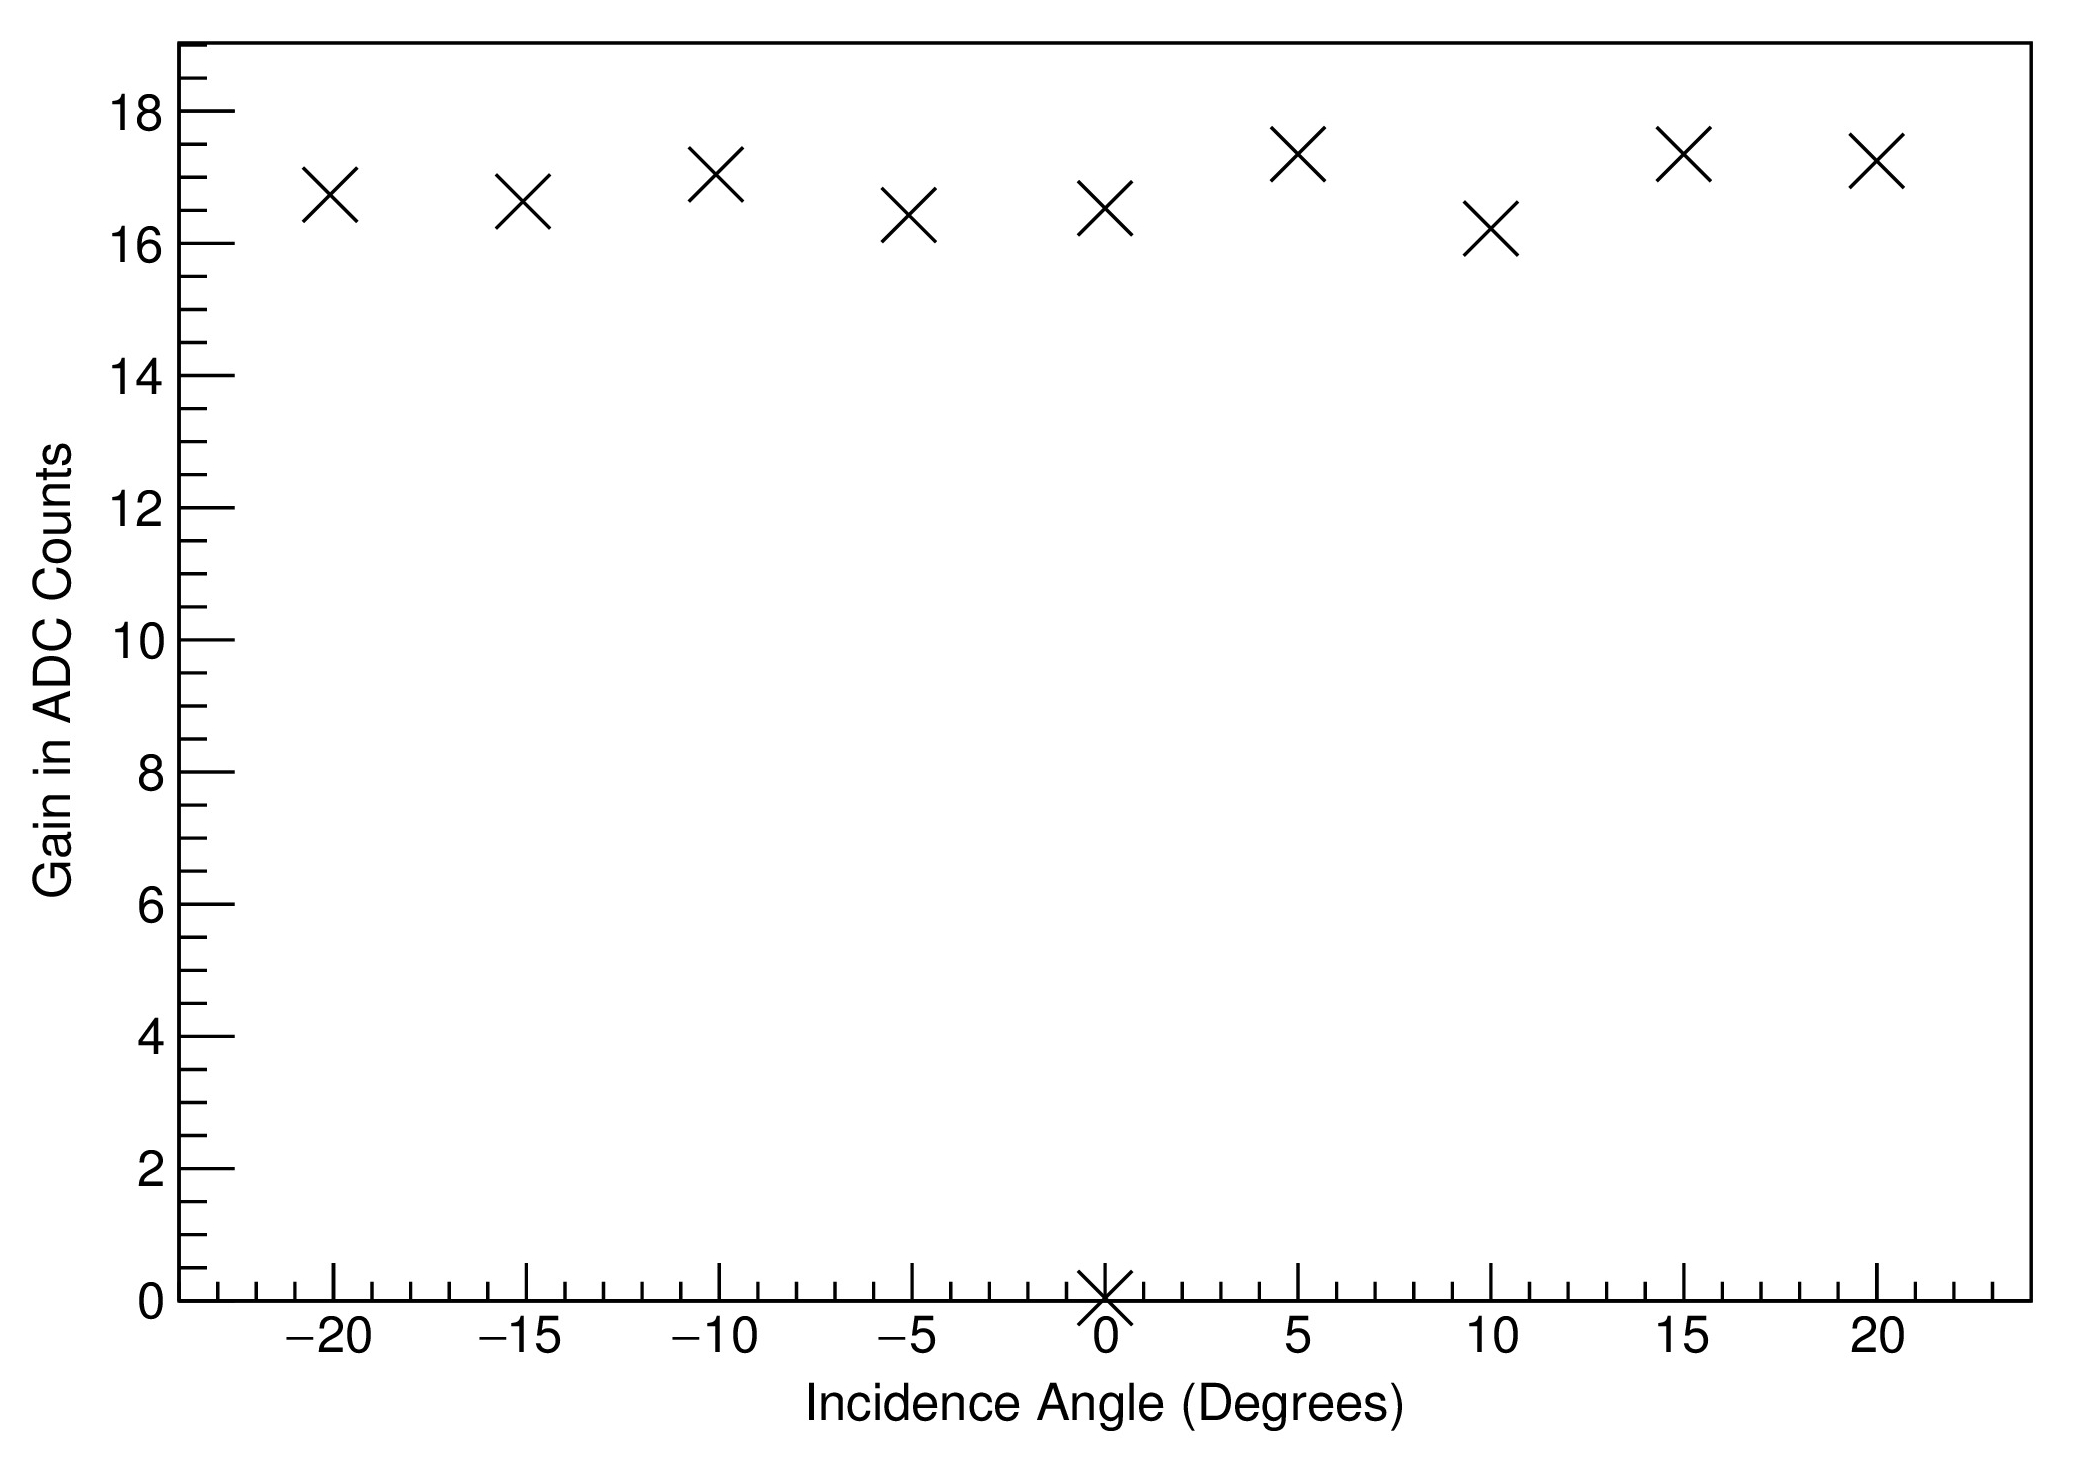
\includegraphics[scale=0.08]{gainAngle.jpg}
	\caption{Gain variation with Incidence Angle}
\end{figure}
\FloatBarrier
\begin{figure}[!htpb]
	\centering	
	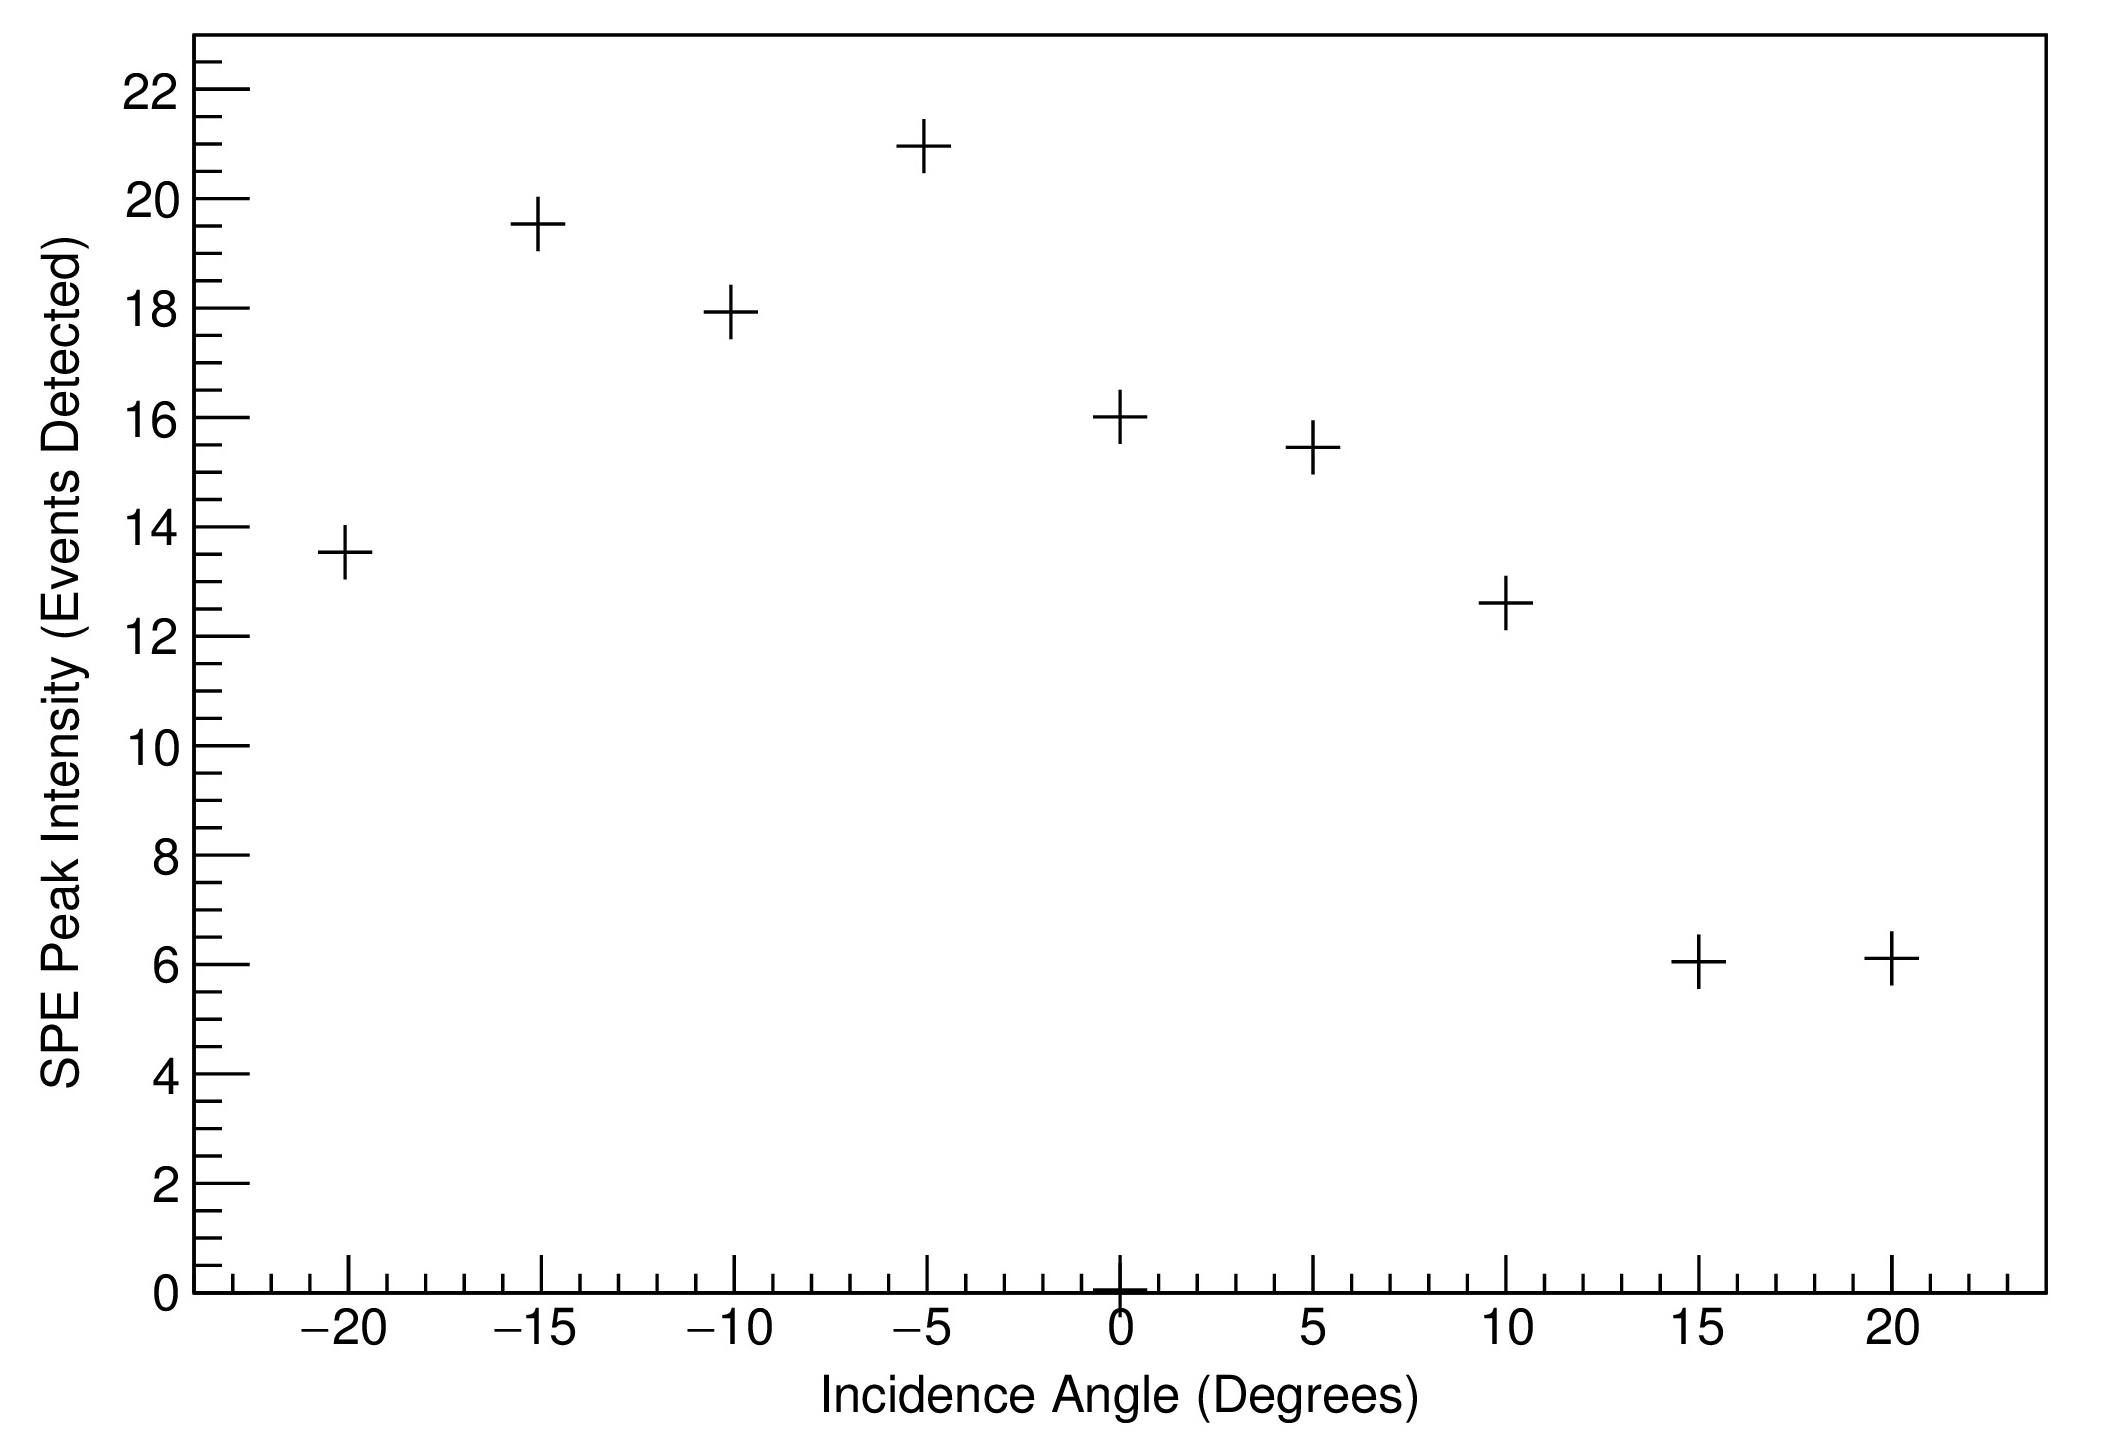
\includegraphics[scale=0.08]{peakIntensityAngle.jpg}
	\caption{SPE Peak Intensity variation with Incidence Angle}
\end{figure}
\FloatBarrier

%\subsection{Magnetic Field Studies}
%
%The location of the PTF in close proximity to the cyclotron at TRIUMF necessitated high precision %control of the ambient magnetic field.  For a variety of cyclotron states and other facility %activities, magnetic field data was obtained using the phidgets in each optical box. As well, full %magnetic field scans were taken of the volume in which the PMT is positioned. 
%
%\subsubsection{Cyclotron Activity}
%
%\subsubsection{Coil Tuning}
%
\section{Discussion}

\subsection{Factors Influencing PMT Response}	

\subsubsection{Gain}

Initial scans of the full PMT surface show strong evidence of gain variation across the PMT surface, as seen in Fig 6, 9 and 10. The magnitude of this gain variation is on the order of $50\%$ relative to the average value across the surface of the PMT.  An earlier paper discussing improvements made to the Hamamatsu R3600 PMT describes a similiar variation in gain of the PMT at various positions across the surface of $\pm40\%$  \cite{PMTImprovement:suzuki}.

Calculation of the gain of a PMT, as defined in \ref{sec:general_analysis}, is based primarily on fitting at Gaussian to the ADC spectrum.  If there is a significant contribution to the spectrum from higher order photoelectron peaks, the fitted Gaussian will be skewed towards a higher gain.  However, the ADC spectra observed in both preliminary scans (Fig 6,9,10) and in the Hamamatsu Improvement Paper \cite{PMTImprovement:suzuki} show minimal contamination from higher order PE emission. More likely, the gain variation and variations in other PMT response characteristics are due to the ambient magnetic field strength and direction, as well as the dynode structure of the electron multiplier circuit. 

Figures 9 and 10 are full PMT surface scans taken at 1cm resolution at an ambient magnetic field of $700mG$. The two scans show similar magnitude of gain variation, however the overall pattern of the gain variation is different. The only variable that was not kept constant between the two scans is the direction of the magnetic field, with the field in Fig. 9 having a positive direction, and the field in Fig. 10 having a negative direction as defined by the Z-axis of the gantry system.

\subsubsection{Incidence and Azimuth Angle}

Preliminary investigation of the effect of photon incidence and azimuth angle on the response of the PMT as shown in Fig. 11, Fig. 12 and Fig. 13 indicate negligible gain variation with changing incidence angle, but large variation in detection efficiency and SPE Peak intensity.  This data suggests that the gain of the PMT is solely dependent on the trajectory of the emitted photoelectron from the photocathode, while the overall detection efficiency for a point on the PMT surface is also a function of the trajectory of the incident photon.  

A caveat to the method used in this preliminary study is the use of tape defining a $1cm\times1cm$ region on the surface of the PMT.  Due to the $1cm$ spot size of the laser incident to the PMT surface it is highly likely that the detection efficiency and SPE Peak intensity measurements include the effect of the geometry of the taped region on the number of incident photons to the surface of the PMT. Future studies will only use the tape for PMT location and incidence angle calibration purposes.

\subsection{Ongoing and Future Studies}

\subsubsection{Gain}

The limited preliminary gain studies strongly suggest a correlation between magnetic field strength and the observed gain variation at points on the PMT surface.  Future studies will be focused on quantifying the effect of the direction and magnitude of the ambient magnetic field on the gain of the PMT, with the goal of understanding PMT behaviour at low field strengths ($<100mG$).

\subsubsection{Incidence and Azimuth Angle}
Final calibration of the incidence and azimuth angle calculation script detailed in \ref{sec:incAngle} is necessary for incidence angle measurements taken without a taped region for locating purposes.  Completion of this final calibration will provide an uncertainty on the incidence angle and position of the incident photons on the surface of the PMT. 

Once completed, a scanning procedure will be developed to scan the PMT surface at a range of incidence angles, allowing quantitative measurement of the response of the PMT to variation of the trajectory of incident photons. 

\section{Conclusion}

Current work in developing a framework for data collection and analysis at the PTF has resulted in a system capable of taking measurements of the response of the entire area of the PMT at a fixed global incidence angle, or an isolated region of the PMT at a varying incidence angle.  Continuing work refining incidence angle calculations, magnetic field control systems and analysis algorithms is necessary, with the goal of producing a system that can quickly, reliably and accurately measure PMT response to a range of varying conditions.  


\appendices
\section{}
Appendix text here.  Some information is beyond the scope of the current version of this document, and so is not included for brevity.  Any reference to the appendix should be seen as a TODO for the final version.

% references section

% can use a bibliography generated by BibTeX as a .bbl file
% BibTeX documentation can be easily obtained at:
% http://mirror.ctan.org/biblio/bibtex/contrib/doc/
% The IEEEtran BibTeX style support page is at:
% http://www.michaelshell.org/tex/ieeetran/bibtex/
%\bibliographystyle{IEEEtran}
% argument is your BibTeX string definitions and bibliography database(s)
%\bibliography{IEEEabrv,../bib/paper}
%
% <OR> manually copy in the resultant .bbl file
% set second argument of \begin to the number of references
% (used to reserve space for the reference number labels box)

\begin{thebibliography}{1}
  
\bibitem{PMTImprovement:suzuki}
Suzuki, A., Mori, M., Kaneyuki, K., Tanimori, T., Takeuchi, J., Kyushima, H. \& Ohashi, Y. (1993). Improvement of 20 in. diameter photomultiplier tubes. Nuclear Instruments and Methods in Physics Research Section A: Accelerators, Spectrometers, Detectors and Associated Equipment, 329(1-2), 299-313. doi:10.1016/0168-9002(93)90949-i

\end{thebibliography}



% that's all folks
\end{document}


